\documentclass[letterpaper,12pt,extrafontsizes,final]{memoir}
\usepackage[pdftex]{graphicx}
\usepackage{amsmath,wrapfig,float,indentfirst,subfig,enumerate,array,threeparttable,longtable} 
%\usepackage{lscape}
\usepackage{pdflscape}
\usepackage{fullpage}
\usepackage{appendix}
\usepackage[USenglish]{babel}       %US hyphenation rules
%\usepackage{setspace,listings,geometry,ltablex,booktabs,tocloft}
\usepackage{type1cm,courier,relsize,siunitx,fixltx2e,alltt,xcolor,mdwlist}% Replace the standard Computer Modern Typewriter font LaTeX uses, monospace text with PostScript font Adobe Courier, use relative sizes(e.g. \smaller, \larger),set SI units correctly
\usepackage{latexsym}
\usepackage[square,comma]{natbib}
\usepackage{citeref}
\usepackage{hyperref}
\hypersetup
{
    pdfpagelayout=TwoPageRight,
    bookmarks=true,           % show bookmarks bar?
    unicode=false,               % non-Latin characters in Acrobat�s bookmarks
    pdftoolbar=true,             % show Acrobat�s toolbar?
    pdfmenubar=true,          % show Acrobat�s menu?
    pdffitwindow=false,        % window fit to page when opened
    pdfstartview={FitH},       % fits the width of the page to the window
    pdftitle={A Study of Real Time Kinematic Global Navigation Satellite Systems In Railroad Transportation},    % title
    pdfauthor={Peter J Dailey},     % author
    pdfsubject={Track Surveying},   % subject of the document
    pdfcreator={Peter J Dailey},   % creator of the document
    pdfproducer={Peter J Dailey}, % producer of the document
    pdfkeywords={RTK,GPS,GNSS,survey,railroad,alinement,alignment,track,occupancy,yard,hump,real-time,kinematic}, % list of keywords
    pdfnewwindow=true,% links in new window
    colorlinks=true,        % false: boxed links; true: colored links
    linkcolor= blue,        % color of internal links, red
    citecolor=black,        % color of links to bibliography, green
    filecolor=black,         % color of file links, magenta
    urlcolor=blue          % color of external links, cyan
}
%
\widowpenalty=500
\clubpenalty=500
\OnehalfSpacing
\tightlists
\setsecnumdepth{chapter} % number to section
%
% Alter some LaTeX defaults for better treatment of figures:
    % See p.105 of "TeX Unbound" for suggested values.
    % See pp. 199-200 of Lamport's "LaTeX" book for details.
    %   General parameters, for ALL pages:
    \renewcommand{\topfraction}{0.9}	% max fraction of floats at top
    \renewcommand{\bottomfraction}{0.8}	% max fraction of floats at bottom
    %   Parameters for TEXT pages (not float pages):
    \setcounter{topnumber}{2}
    \setcounter{bottomnumber}{2}
    \setcounter{totalnumber}{4}     % 2 may work better
    \setcounter{dbltopnumber}{2}    % for 2-column pages
    \renewcommand{\dbltopfraction}{0.9}	% fit big float above 2-col. text
    \renewcommand{\textfraction}{0.07}	% allow minimal text w. figs
    %   Parameters for FLOAT pages (not text pages):
    \renewcommand{\floatpagefraction}{0.7}	% require fuller float pages
	% N.B.: floatpagefraction MUST be less than topfraction !!
    \renewcommand{\dblfloatpagefraction}{0.7}	% require fuller float pages
% remember to use [htp] or [htpb] for placement
\usepackage{graphicx}
\usepackage{epstopdf}
\DeclareGraphicsRule{.tif}{png}{.png}{`convert #1 `dirname #1`/`basename #1 .tif`.png}
\begin{document}
%
\frontmatter
	\thispagestyle{empty}
\begin{center}
\DoubleSpacing
\Large
A STUDY OF \\
REAL TIME KINEMATIC\\
\mbox{GLOBAL NAVIGATION SATELLITE SYSTEMS}\\
IN RAILROAD TRANSPORTATION\\
	 \vspace{80pt}
% Author
	\large{by\\\textsc{Peter Joseph Dailey}}\\ \vspace{40pt}
	A Research Proposal Presented In Partial Fulfillment\\
	Of The Requirements For The Degree\\
	DOCTOR OF PHILOSOPHY\\
	IN CIVIL ENGINEERING\\
	 \vspace{80pt}
% Bottom of the page
	\large{WEST VIRGINIA UNIVERSITY\\\today}
\end{center}

		\cleardoublepage
	\thispagestyle{empty}
\begin{center}
	\large{ A STUDY OF \\
	REAL TIME KINEMATIC\\
	\mbox{GLOBAL NAVIGATION SATELLITE SYSTEMS}\\
	IN RAILROAD TRANSPORTATION}\\
	 \end{center}
% Author
\begin{center}
\vspace{6pt}
\textsc{Peter Joseph Dailey}\\
\SingleSpacing A Research Proposal Submitted to the Graduate\\
Faculty of West Virginia University\\
in Partial Fulfillment of the\\
Requirements for the Degree of\\
Doctor of Philosophy\\
Major Subject: Civil Engineering
% Committee
\vspace{20pt}\\
PROPOSAL COMMITTEE\\ 
\vspace{50pt}
\begin{tabular}{c c c}
&  &  \\
\hline
&David R. Martinelli, PhD, chair&\vspace{40pt}\\ \hline
&Darrell R. Dean, PhD&\vspace{40pt}\\ \hline
&Jim French, PhD&\vspace{40pt}\\ \hline
&Andrew Nichols, PhD&\vspace{40pt}\\ \hline
&Avinash Unnikrishnan, PhD \\
\end{tabular}
\end{center}
		\cleardoublepage
	\include{abstract}
		\cleardoublepage
	\include{acknowledgements}
		\cleardoublepage
	\begin{center}
\chapnamefont{Dedication}\\
\end{center}
\vspace{40pt}

This research is dedicated to the men and women of the railroad industry that go to work thinking of their own and of their coworker's safety; perform their duties while remembering to work safely; and at the end of each shift, return safely home to their loved ones. Then, wake up and do it all again, every day.
		\cleardoublepage
	%\preface{preface}
	\tableofcontents
	\listoftables*
	\listoffigures*

\mainmatter
	% !TEX root = dissertation2.tex
\chapter{Introduction}
The shipment of freight by rail is an exceptionally fuel efficient transportation mode. The average freight train consumes one gallon of diesel fuel to move one ton 423 miles~\citep{RITAtransStats08}. The outstanding efficiency of rail freight comes with a high price in inspection and maintenance of the railway. Rail car loading forces, weather, and time act on the railway and substructure to distort the track geometry. Distortions to the track geometry\footnote{i.e., gage, profile, alinement, crosslevel, superelevation, and warp.} must be identified and maintenance resources brought to bear to insure safe operation at the design track speed. 

FRA\footnote{Federal Railroad Administration} mandated visual track inspections rely on a rail company inspector's training, skill, and diligence. Conversely, track geometry car inspections provide an objective, detailed record of relative track position but are performed infrequently due to the limited availability of these specialized measurement systems. The thesis of this research is that, given a sufficiently accurate and reliable augmentation system, railway infrastructure measurement can be performed quickly, with greater safety, and at less cost by determining absolute track position using global satellite positioning systems. Survey-grade track measurement using GNSS\footnote{Global Navigation Satellite Systems} instrumentation will remove ground-based surveyors from the hazards inherent to active rail yards; enable monitoring of rail position changes during routine visual inspections; and determine the track occupancy of a train in parallel multi-track segments in signalized or dark territory\footnote{No signal control}, independent of wired track circuits.

The research results present an investigation into the use of Real Time Kinematic (RTK) augmentation to global satellite navigation systems in the measurement of absolute track position. Survey quality track positions enable the development and demonstration of solutions to rail measurement in an active hump yard and across 29 continuous miles of parallel mainline track.

Space vehicles (SV) that comprise the GPS\footnote{Sponsored by the United States Department of Defense (USDOD)}, as well as other global navigation satellite systems: GLONASS\footnote{GLObal'naya NAvigatsionnaya Sputnikovaya Sistema  sponsored by the Russian Space Forces}; Galileo\footnote{Sponsored by the European Union}; and the future CNSS\footnote{Compass Navigation Satellite System proposed by the Peoples Republic of China}, are orbiting reference beacons enabling autonomous geo-spatial positioning and timing across the globe. The geo-spatial positioning accuracy of these systems can be improved by augmenting the identifiable distortions to SV signal transmissions through the ionosphere and troposphere with corrections from ground based facilities. 

The use of GPS positioning for rail infrastructure measurement has depended on federal government supplied augmentation. The United Stated Department of Transportation (USDOT) has selected the National Differential GPS (NDGPS) augmentation system to increase accuracy in transportation applications. NDGPS has been promoted by the FRA as a means to achieve reliable track occupancy, however no NDGPS equipment demonstrating the requisite accuracy or reliability to insure track occupancy has been publicly disclosed~\citep{2006AllenAssetMap}. The FRA reported in 1995 that ``When [track occupancy is] viewed as a two dimensional area problem, it is unlikely that any economically feasible [GPS] system could achieve this accuracy to the required $0.9_5$\footnote{0.99999 or 99.999\%} probability~\citep[pp.6-7]{1995FRADiffe}.'' The economically feasible reference is interpreted here to mean the existence of commercial off-the-shelf (OTS) technology.

% Problem Statement
% Motivate the problem through time, money, safety
% Benchmarks that motivate the study
% Identify the weak link in the system
% Research questions are previewed int the problem statement
% By solving the problem we will answer these research questions

\section{Railway Measurement Problems}
Track course smoothness must be held within specific tolerances to avoid undesirable lateral accelerations that lead to additional railway distortions and derailment. A system for track surveying should be cost-effective, provide relative accuracy without interfering with train traffic, and minimize worker exposure to railway hazards. Historically, North American railways use relative measurement methods for track inspection. Track course measurement is based on the idea that track degree of curvature ($D_c$) irregularity can be determined by the versine\footnote{In rail transportation, versine refers to relationship between the distance ($v$) measured at right angles from the midpoint of a chord ($L$) to the arc, with the instantaneous  $D_c$ determined from $\displaystyle\lim_{L\to0} 8\frac{v}{L^2}$}~\citep{Nair}(see figure \ref{fig:Alinement}).

The research applies augmented GNSS to measure track elevation in a hump yard for the purpose of track profile measurement; measuring track horizontal position in order to determine the $D_c$ of mainline track across a wide area; and determining track occupancy probability independently of wired track circuits. Three railway measurement problems were investigated during the research.
\begin{enumerate}
\firmlist
	\item An automatic classification yard uses the force of gravity to propel cars through a complex system of tracks to the intended destination in the yard. Environmental factors\footnote{Wind speed, direction, and ambient temperature} act on the motion of a railcar from its release, through a transit of specific yard tracks, to a final rest position. Profile deviation from the design grade occurs over time from settlement as a result of railcar loading forces and the effects of weather~\citep{2005szwilski}. Conducting a differential level survey across a 60 track, thousand car per day yard, places workers in harms way, making yard production delays unavoidable in order to accommodate the safety of the survey party. The difficulty and expense in conducting a yard survey to quantify production delays attributable to grade irregularities can be prohibitive~\citep{2007barnes}. 
	
A hump yard profile survey was conducted by locomotive equipped with RTK GPS survey instruments. The survey was conducted during production, inclement weather resulting in the production of 58 track profiles.
	
	\item Track superintendents rely on an occasional traverse by a specialized track geometry car and routine visual inspections to identify track defects for directing maintenance resources. A method of recording track alinement during routine visual inspections by Hi-Rail and producing a record of track alinement provides insight into the identification of track shift or compliance irregularities attributable to car loading, weather, or geologic processes.
	
COTS surveying instruments and infrastructure were used during a track inspector's normal visual inspection by Hi-Rail to determine degree of curvature ${D_c}$. A instrument mounted to a Hi-Rail recording track position across a track inspectors 29 mile area of responsibility. A software modeling the string lining method~\citep{49CFR213D,2007FRATrack,2009bright}(hereafter referred to as \emph{the model}) determined ${D_c}$ and mile post reference locations. The RTK Hi-Rail $D_c$ were compared against rail company track charts to verify the model. The accuracy of the Hi-Rail method of determining $D_c$ was compared against measurements by a specialized track inspection vehicle.
	
	\item Locating a train in a parallel, multi-track segment by means of GNSS requires a priori knowledge of each track segment's location. The present US rail transportation system inventory of 95,000 mainline track miles makes monumenting the absolute location of each track centerline to a high degree of accuracy a formidable task. Most rail company's have chosen LiDAR overflights to monument the position of track and wayside assets.
	
	A track vehicle using wireless position measurement determined a reference track centerline location against which subsequent traverses by the track vehicle where compared. Subsequent track positions met the researcher's interpretation of the FRA positioning guidlines for a location determination system (LDS) as might be used for positive train control (PTC)~\citep[pp.3]{1995FRADiffe}.

\end{enumerate}  

% Objectives can provide a certain standard for measurement
% Track inspection motivates the research

\section{Research Questions}
The researcher sought to wirelessly assess railway infrastructure and use wireless location to act as a reliable track vehicle locator. 

The solution to many track measurement and rail vehicle location problems requires absolute track and vehicle position measurement over wide areas. The research integrated wireless track measurement within the operational and safety constraints of a Class I rail company for the purpose of developing a method to survey track location with common track vehicles. The rail transportation problems addressed by the research seek to decrease on-track worker hazard exposure, increase track inspection efficiency, and reduced the cost of track measurement. The research employed locomotives and HiRail vehicles equipped with COTS survey equipment to evaluate the relative vertical precision, horizontal accuracy, and position reliability of RTK augmentation. The research used a wireless measurement system to meet the ``...high integrity, and high reliability for safety-critical train control applications~\citep[pp.11]{2008USDoT_NDGPS}.''

Objectives of the research developed procedures and supporting models for assessment of wireless track measurement integration within a Class I railroad environment.
\begin{enumerate}
\firmlist
\item A literature review of previous rail survey experimental results as well as a search of intellectual property claims regarding train location were used to investigate factors that indicated the need for research into the wireless measurement of railway position. The review was used to determine a wireless method using COTS instruments with sufficient accuracy to meet the measurement goals.
\item Experts in the field of hump yard engineering were interviewed, and a review of the literature was used to identify methods of increasing humpyard efficiency and throughput. Railcar motion was studied through a humpyard in an effort to identify operational problems that may be related to profile degradation.
\item A method was developed and demonstrated to safely and precisely determine track grades across the bowl area of an automatic classification yard. The selected wireless method was used to produce individual profiles for each bowl track in the yard. The relative vertical precision of the mobile receiver and the signals recorded by a reference station in the yard were evaluated for evidence of signal distortions in the hump yard environment.
\item Experts in the field of track inspection and wide area RTK augmentation delivery were interviewed to identify methods for measuring rail position over wide areas of mainline track.
\item A method was developed and demonstrated for safely determining horizontal track alinement across a wide area.
\item A model was developed to determine horizontal track alinement based on the string lining method using RTK GNSS observations. Factors affecting GNSS measurement over mainline track were analyzed.
\item A methodology was developed to assess wireless measurement methods as part of a location determination system suitable for supporting positive train control. COTS RTK GNSS VRS infrastructure and instrumentation were evaluated in parallel multi-track mainline segments for the ability to meet FRA tolerances~\cite[4-5]{1995FRADiffe}.
\end{enumerate}

% Research Contribution
%Significance
Development and demonstration of wireless method of track position is significant to providing the rail industry with a practical and reliable standard for rail position measurement over a wide area. Several tools were developed enabling a solution to railway infrastructure measurement and monitoring problems that has not been demonstrated with US government provided GPS augmentation. Intelligent rail transportation initiatives will benefit from survey-quality positioning in the command, control, communications, and track information domains. Freight transportation will derive benefit from  improved power and braking systems which will result in improved energy efficiency and decreased emissions; improved systems for track defect detection and track movement prediction; improved efficiency in the deployment of maintenance assets; examination of track substructure through determination of the track modulus between lightly loaded (as with a HiRail) and loaded (as with a locomotive) track measurements; and safety improvements derived from Positive Train Control (PTC) systems with the potential to significantly reduce the probability of collisions between trains, casualties to roadway workers, damage to equipment, and reduction in the occurrence of overspeed accidents through the wireless differentiation of track vehicle location over parallel multi-track segments.

Reliable wireless measurement of track position, when contrasted with the present use of dedicated track circuits\footnote{i.e., insulated track circuits, loop detectors, magnetic proximity switches, transponders}, provides and opportunity to use wireless measurement technology to enhance railway infrastructure management practices. Track vehicle location and control benefits from survey quality wireless measurement, coupled with the use of existing wayside radio infrastructure, has the potential to provide economic benefit by reducing a rail company's dependance on existing hard-wired infrastructure\footnote{Estimated replacement mainline cost of \$125,000 per mile $\times$ 95,000 miles = \$12 billion~\citep{ResorPTC}} and attendant labor costs.

Other cited benefits of accurate train location may include:
\begin{itemize}
\firmlist
	\item Higher quality service, through continuous tracking of car movements.
	\item Reduced fuel consumption, through better pacing of trains (avoiding the need to take away momentum through braking and restore it through use of diesel power).
	\item More efficient use of existing physical plant, increasing effective capacity while avoiding further outlays to build additional tracks or sidings.~\citep[pp.12-13]{1995FRADiffe}
\end{itemize}

% Operational Definitions
\section{Operational Definitions}

\begin{enumerate}
\firmlist

	\item Hump yard: This study specifically refers to the Hamlet Terminal, owned by CSX and located in Hamlet, North Carolina.

	\item Mainline track: A track extending through yards and between stations which must not be occupied without authority or protection. This study refers to mainline track as C\&O Ohio Subdivision from mile post (MP) 211 to MP 207 (Guyendotte, West Virginia), and C\&O Kanawha Subdivision from MP494 to MP 523 (Barborsville, WV to Russell, KY).

	\item Mapping-grade accuracy: An observed position within 3-16 feet (1-5 meters)  horizontally and 6-33 feet (2-10 meters) vertically of the true value with 95\% confidence.

	\item Survey-grade accuracy: The combined measurement errors from instrumentation and the measurement process producing a position to within 0.1 feet or less of the true value in the horizontal and vertical plane with 95\% confidence.

	\item Track occupancy: FRA LDS guideline for differentiating between parallel tracks with a 11.50 foot centerline-to-centerline track spacing using GPS. The FRA track spacing requirement is interpreted in this study as a point obtained from a mobile track vehicle no greater than $\pm\frac{11.50}{2}$ feet left(-) or right(+) of a track centerline with 99.999\% confidence~\cite[pp.6-7]{1995FRADiffe}.

\end{enumerate}

\section{Research Questions}
The research conducted in this investigation was an analytical study
supplemented by the acquisition of wireless track observations. The research focused on the integration of RTK augmented GNSS within the operational constraints of a Class I railroad. As a result of this research, a methodology for the assessment of railway infrastructure was developed.

The problems solved by the determination of absolute track location to a high degree of accuracy in a hump yard and over mainline track answered these questions.

1)\emph{Hump Yard Profile:}
Can a locomotive use wireless position measurement to determine the vertical profile of bowl tracks in an automatic classification yard to an accuracy of tenth of a foot during production activities?

2)\emph{Horizontal Track Alinement:}
Can a common track vehicle use wireless position measurement to determine the horizontal degree of curvature ($D_c$) comparable with specialized track geometry vehicles?

3)\emph{Track Occupancy:}
Can a common track vehicle use wireless position measurement to meet the FRA~\citep[pp.6-7]{1995FRADiffe} accuracy and confidence guidelines for track occupancy as might be used in a location determination system?


	% !TEX root = dissertation2.tex
\chapter{Literature Review}
The literature review supported answering these research questions:

1)\emph{Hump Yard Profile:}
Can a locomotive use wireless position measurement to determine the vertical profile of bowl tracks in an automatic classification yard to an accuracy of tenth of a foot during production activities?

2)\emph{Horizontal Track Alinement:}
Can a common track vehicle use wireless position measurement to determine the horizontal degree of curvature ($D_c$) comparable with specialized track geometry vehicles?

3)\emph{Track Occupancy:}
Can a common track vehicle use wireless position measurement to meet the FRA~\citep[pp.6-7]{1995FRADiffe} accuracy and confidence guidelines for track occupancy as might be used in a location determination system?

\section{Manifest Freight and Hump Yard Efficiency}
Car load freight traffic requires a systematic method for handling the distribution of car destinations, the return of empties, and redirecting cars to their originating industry. On-time delivery in carload service requires minimizing delay during a series of independent car handling events. Beshers notes that each transit through a terminal decreases the probability of an on-time delivery, and provides a statistical determination of overall freight service reliability as the product of the probability-of-delay each time a car is handled along the way to its destination~\citep{2004beshers}. Moorman points to the difficulty rail freight carriers have in achieving acceptable carload service levels in retaining market share~\citep{2006moorman}.

Automated classification yards\footnote{Commonly referred to as hump yards.}, are facilities engineered to continuously process incoming freight cars into outbound trains. Car processing in a hump yard uses the force of gravity to propel cars through a complex of tracks to the intended destination in the yard.

Beshers point to the degradation of car-load service quality and movement away from boxcars to inter-model freight as factors that have resulted in a clear trend towards rail company closure or repurposing of hump yards rather than investing in new facilities~\citep{2004beshers}. Several older hump facilities remain in use but have been repurposed as flat switching yards, as in Russell, KY, Dewitt, NY, and Enola, PA. Others have been converted into intermodal facilities, such as Norfolk Southern Atlanta, GA and Rutherford, PA yards~\citep{2002HumpTrains}.

Dr. Edwin Kraft in a patent claiming to increase yard throughput through a multi-stage sorting algorithm, points out that surviving hump yards operate at close to maximum throughput and operate under a state of constant congestion, to the point that they often cannot accept newly arriving trains. In these circumstances cars are parked on main line track and wait to be processed. Hump yard congestion affects rail service reliability across the network, which in turn contributes to further loss of rail traffic to the trucking industry~\citep{KraftPaten00}.

A hump yard's profile deviation and settlement away from the design grade can be attributed to the effects of car loading forces and weather. Szwilski and Kerchof's observation that yard delays attributable to grade irregularities are difficult to identify due to limited yard profile data available to the hump yard engineer~\citep{2005szwilski}. When interviewed, Barnes echoed Szwilski and Kerchof in noting that the limited availability of profile data is due primarily to the difficulty in conducting a survey to profile track~\citep{2007barnes}.

Szwilski and Kerchof estimated a differential level survey across a 72-track hump yard would take 4 to 6 weeks of field work by a three-person survey crew. A differential level survey point density is typically measured on 100' stations, resulting in the observation of approximately 3,000 points within the bowl area of the yard. An estimated 480 to 720 man-hours of exposure to rolling stock in an active yard evidences the need to insure the survey party's safety by closing groups of tracks to production activity. Extended track closures require rerouting railcars away from the yard to prevent yard congestion. The associated cost to reroute railcars is difficult to estimate~\citep{2005szwilski}. Safety consideration for the survey party require the yard manager to dedicate specifically trained workers from the yard's labor pool to act as a safety escort. The specter of six continuous weeks of negative production due to track survey activity limits a manager's tolerance for obtaining track profiles, no matter how well intentioned the survey intrusion~\citep{2007barnes}.

The hump end of an automatic classification yard controls the motion of a railcar through the yard. Hump end yard operations are described visually in \href{http://www.youtube.com/watch?v=ndryMwF41Kk}{this video}\footnote{$http://www.youtube.com/watch?v=ndryMwF41Kk$} and provide a graphic understanding of railcar pacing, car variety, and braking~\citep{HumpOpsVid}. The video follows several railcars from release by the pin puller, through the main, intermediate, and group retarders, passing lead and group switches into the bowl to couple at a controlled speed intended to be no greater than 4 mph. The requirement for personal protective equipment in or near a hump yard is obvious from the retarder/wheel flange squeal in the audio track.

Anecdotal inference of yard infrastructure problems is the usual mechanism by which grade renewal is scheduled. An experienced observer might use the reaction of a car's truck and bolster as an aid in revealing underlying track irregularities.

Modern hump yard control systems, such as the ProYard and ProYardII systems, are able to count car transits through the yard network as cars pass wheel detectors (magnetic proximity switches) linked to  PLCs\footnote{Programable Logic Controllers} programmed with timing logic. Misroutes and car stalls recorded by modern hump control systems are metrics used to gauge overall yard performance as well as distinguishing individual track irregularity.

A \href{http://www.youtube.com/watch?v=ygl_X9RER70}{time lapse video}\footnote{$http://www.youtube.com/watch?v=ygl_X9RER70$}~\citep{CarStallVid} shows a series of stalled flatcars. The opening frames show a flatcar moving away from the hump, striking a group of stalled flatcars. As a result of insufficient coupling speed, the flatcar rolls back toward the hump, with the car's final rest position blocking the group switch. The blocked switch prevents any additional railcars from classification into the blocked group. The stall effectively shuts down humping operations when the next car sequenced for the blocked group reaches the pin puller. The time-lapse sequence from stall to the trim locomotive kicking the cars into the alley represents 21 minutes of delay, indicative of the cumulative effects from profile-induced delay affecting the on-time quality of car load service.

% Radio-reflective environment
An FRA sponsored study examined the effects of locomotive electromagnetic fields on the NDGPS signal, finding a reduction of some 10db in particular antenna configurations~\citep{2000FRA_gps_ant}. Radio-reflective structures and the metal railcars may affect GPS signals in a hump yard. GPS signal reflections from fixed an moving surfaces present an opportunity to introduce complex multipath distortion to GPS receiver, in addition to the effect of electromagnetic fields generated by a locomotive from the generator and traction motors.

\section{Absolute Track Location Measurement Systems}
% Theory and research specific to the topic
% \section{Theory/research specific to the topic}
The ``other supplemental techniques'' referenced in the USDOT NDGPS Assessment are reflected in patents that integrate differential GPS, inertial systems, and wheel mounted tachometers to produce optimal estimators for determining locomotive track occupancy~\citep{2007lockheed}. Supplemental techniques were demonstrated across a wide area of mainline track in an asset mapping system demonstrated by Allen, Mason, and Stevens.

Allen, Mason, and Stevens developed a rail borne track-mapping system as a cost saving alternative to remote sensing from an aerial platform. Their survey platform consisted of a HiRail vehicle equipped to utilized publicly available real time correctors from the NDGPS in addition to post processed observations from a cooperative\footnote{http://www.ngs.noaa.gov/CORS/Coop/} Continuously Operating Reference Station (CORS). The GPS instrument was augmented with tachometer and inertial measurement unit (IMU) inputs. Allen reported that an initial calibration on a dedicated survey vehicle took two days.

Rail positions measured by Allen's HiRail were compared against 26 centerline targets previously surveyed using RTK GPS. NDGPS correctors were available during 80\% of the 120 mile traverse of Norfolk Southern mainline track. Two Post-Processed Kinematic (PPK) positions were divided into two categories by distance to the CORS. A first category of observations was processed against a CORS at under 65 miles distant from the survey vehicle, with a second category of PPK positions processed against a CORS between 65 and 130 miles distant from the survey vehicle.

% Table of results: Allen
\begin{center}
\begin{threeparttable}
	\caption{Track Measurement Results~\citep{2006AllenAssetMap}}\label{tab:Allen}
		\begin{tabular}{ lcccc }
		\toprule
		Measurement &  Cross-Track\tnote{*} & Along-Track\tnote{*} & Elevation\tnote{*} & Absolute\tnote{*}\\
		\midrule
		NDGPS & 5.2418 & 5.4766 &13.5308 & 8.0834\\
		%\midrule
		PPK $<$ 65~mi. & 1.5758 & 1.4766 &4.4049 & 1.8917\\
		%\midrule
		PPK 65$-$130~mi.  & 2.9084 & 2.5003 &10.2528 & 3.8505\\
		\bottomrule
		\end{tabular}
		\begin{tablenotes}
		\item[*]{Feet, 95th percentile. Significant figures reported by Allen.}
		\end{tablenotes}
\end{threeparttable}
\end{center}

The cross-track differences between previously surveyed RTK track locations and those measured by HiRail summarized in table \ref{tab:Allen}. No determination for LDS suitability was reported.

% Allen Cross track diagram
\begin{figure}[!htp]
\begin{center}
	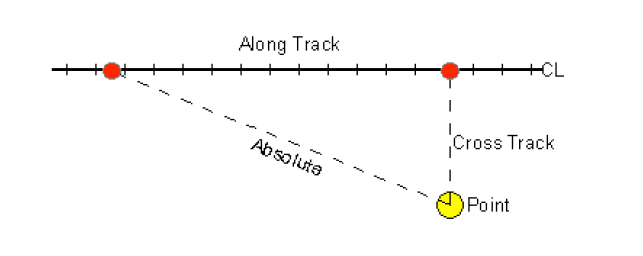
\includegraphics[width=3in]{graphics/AllenTrackRef.png}
	\caption{Track Centerline Accuracy Parameters~\citep{2006AllenAssetMap}}
	\label{fig:trackRef}
\end{center}
\end{figure}

Other track asset mapping systems exist for determining the location and type of of assets held by railroads. The Union Pacific Railroad has developed and markets a HiRail-based measurement vehicle built on a SUV chassis and referred to as the Precision Measurement Vehicle (PMV). The PMV is used to provide location and description of all assets that can be measured from the railway. While occupying active mainline track, PMV operators use several measurement technologies to determine asset location. Four independent encoded wheels provide linear referenced track position inputs by by accumulating the slope distance between wayside monuments. A differential GPS receiver provides mapping-grade absolute position, while a fiber optic gyroscope (OG) is used to measure grade. The OG also serves to dampen the elevation observations from the DGPS receiver. A video interface provides the operator with a view through optical distance measuring instruments. A video recorder provides a record for milepost tracking and a survey log. Comparative positions generated by the PMV were not available for examination~\citep{2008pmv}.

Glaus details the development of a lightweight multi-sensor track surveying platform. The 99-pound (45 kg) hand-propelled device, nicknamed the \emph{Swiss Trolley}, tested several sensors and the development of a rigorous mathematical model for calculating kinematic track location. Close tolerance rail alinements are required for high speed passenger rail service. The \emph{Swiss Trolley} fills the need for precision track surveying by demonstrated the ability to determine absolute track axis\footnote{Referred to here as centerline top-of rail.} position to a high degree of precision. The \emph{Swiss Trolley} sensor suite is summarized in table \ref{tab:SwissTrolley}.

% Table of instruments: Glaus
\begin{table}[ht]
\begin{center}
	\caption{Swiss Trolley Instruments~\citep{2006glaus}}\label{tab:SwissTrolley}
	\begin{tabular}{ lll }
	\toprule
	Measurement & Sensor & Range/Resolution\\
	\midrule
	Absolute position & RTK GPS Total Station & 1 mm [sic]\\
	Absolute/relative position & Tracking Total Station & 1 mm\\
	Linear distance & Odometer & 0.08 mm\\
	Cross level/Grade & Inclinometer & $\pm$15$^{\circ}$\\
	Asset location & Laser scanner & 180$^{\circ}$\\
	& & 1 mm @ 32 m\\
	& & 10 mm @ 80 m\\
	Gauge & Angular transducer/rail contact & 0-45$^{\circ}$ \\
	\bottomrule
	\end{tabular}
\end{center}
\end{table}

Analog sensors on the \emph{Swiss Trolley} are linked to a control and data acquisition computer by means of an analog to digital multiplexor. Sensors are synchronized with 1 pps timing pulses generated by the GPS receiver. The sensor suite provides inputs to the model to calculate track axis, grade, cross level, and gauge. Points of concern are raised by the author in dealing with thermal and electrical noise on the analog-to-digital (ADC) converter inputs from a variety of sensors. Electromagnetic compatibility interaction between instruments was addressed by reducing the length and attention to the orientation of cables between sensors and ADCs. Two fluid-damped pendulum sensors provide cross-level and grade inputs. These inclinometers are subject to errors from nuisance vibrations, temperature, and collimation (axis alignment) error. Thermal instability errors were reduced by installing the sensors in an instrument oven to maintain a constant temperature regardless of ambient conditions. Grade and cross-level sensor vibration is modeled as a pendulum and applied to track position corrections. Significant is Glaus's method of integrating auxiliary instruments using Kalman filtering techniques to produce spatial accuracies in the range of several millimeters in a complex dynamic application.

The \emph{Swiss Trolley} is capable of producing exceptional track position accuracies, but the hand propelled sensor suit is limited to a maximum speed of 3.3 mph. Survey speeds are intentionally kept at a minimal to reduce sensor synchronization uncertainty for the platform. The reduced rate also aids in providing an accurate absolute time tag for kinematic data collection~\citep{2006glaus}. In its present form, the tight instrument integration and slow survey speed of the \emph{Swiss Trolley} make this approach impractical for track inspections across wide areas.

\section{Mainline Track Horizontal Alinement}Mainline railways are periodically inspected with specialized ``track geometry cars'' for compliance with FRA mandated track alinement criteria or to meet more stringent rail company specifications~\citep{49CFR213D}~\citep{2009bright}. Alinement data recorded by a track geometry car determines position by use of an odometer for track location within a linear reference system relative to wayside monuments. Wayside references commonly referred to as mile posts range from permanent cast concrete to steel signposts inserted into the ballast. Mile markers are subject to destruction or displacement from routine track maintenance and vandalism. Resetting mile posts is many times a best guess effort. Track geometry car measurements are typically referenced to these reference marks. Track defects referencing offsets from these marks are sometimes difficult to locate by Hi-Rail odometer.~\citep{2009vanPelt}.

The linear measurement system of a track geometry car produces accurate relative positions in the search to alinement defects. A geometry car will use GPS to provide a global reference frame to map alinement exceptions, however the accuracy of these GPS measurements are not adequate for use as a primary alinement tool. Track geometry vehicle inspections are limited in frequency due to the number of vehicles available, with those focused on higher traffic  segments.~\citep{2009bright}.

\section{Track Occupancy}The FRA has established that any location determination system suitable for supporting positive train control must establish track occupancy with a very high degree of certainty. In a given parallel, multitrack segment, an LDS must be able to determine which track a given train is on without error. The FRA therefore requires a LDS to demonstrate track position that assumes a minimum track separation (center to center spacing) of 11.5 feet with 99.999\% confidence~\citep[4-5]{1995FRADiffe}.

A method of autonomous locomotive location referenced by US patent 6,641,090 and follow on 7,209,810 \emph{Locomotive Location System and Method} disclose an apparatus integrating inertial navigation, GPS, and a wheel mounted odometer as a method by which track occupancy can be determined by a train traveling proximal to a turnout. The patent claims teach that the method is able to determine track occupancy when a locomotive travels through a turnout by engaging a Kalman filter to process noisy inputs from accelerometers orthogonal to the direction of travel as the locomotive is diverted from the tangent track into a turnout. The output is compared with predefined track parameters by computing the location and corresponding estimated error states derived from the inertial navigation system until the estimated error state matches a pre-determined feature, indicating the track for that instance is not the track occupied by the locomotive. The method does not teach how to distinguish track occupancy between parallel trackways~\citep{2007lockheed}.

Improving the USDOD\footnote{United States Department of Defense} guarantee of  12.8 meter horizontal accuracy from the Global Positioning System Standard Positioning Service requires that positions calculated by a GPS receiver be augmented to correct for delays induced in the SV\footnote{Space vehicle} signal's travel through the ionosphere and troposphere and a variety of instrument errors~\citep{2001DoDGPSperf}. Correctors transmitted to and processed by a capable receiver are able to compensate for errors and improve the position determined at the receiver's antenna. Correctors are derived from the difference between the instantaneous position calculated at a stationary reference receiver antenna and the actual location of the stationary antenna. The reference receiver determines the signal error for each SV in view of the antenna. The position differential is the product of all ``signals in space'' errors induced in the signal, zeros the clock error between the reference and mobile reciever. SV signal errors accumulate from orbit irregularities (i.e.\ gravitational effects, solar wind, or outdated ephemerides); satellite and receiver clock errors; ionospheric and tropospheric delay; and other identifiable factors~\citep{2004leick}. The reference and mobile receivers must receive the same SV signals for correctors to have an effect on the mobile receiver position accuracy~\citep{2008USDoT_NDGPS}.

Current federal government augmentation systems, the Wide Area Augmentation Systems (WAAS) sponsored by the Federal Aviation Administration and the National Differential GPS (NDGPS) sponsored by the US Coast Guard, provide civilian users with mapping-grade\footnote{Defined here and generally accepted as 1 to 3 meter horizontal accuracy} position accuracy. The USDOT\footnote{United States Department of Transportation} was given presidential authority to develop and promote the use of civilian GPS augmentation systems. 

%USDOT authority for GPS in transportation applications
Presidential Decision Directive National Science and Technology Council (NSTC-6), designating USDOT to serve as the lead agency within the U.S. Government for all Federal civilian GPS matters. NSTC-6 commissioned the USDOT to:
\begin{quotation}
``Develop and implement U.S. Government augmentations to the basic GPS for transportation applications.
\begin{itemize}
\firmlist
	\item In cooperation with the Departments of Commerce, Defense and State, take the lead in promoting commercial applications of GPS technologies and the acceptance of GPS and U.S. Government augmentations as standards in domestic and international transportation systems.
	\item In cooperation with other departments and agencies, coordinate U.S. Government-provided GPS civil augmentation systems to minimize cost and duplication of effort~\citep{1996NSTC-6}.''
\end{itemize}
\end{quotation}

Federal government provided GPS\footnote{Non-GPS augmentation to GNSS systems is not provided by federal government systems} signal augmentation can be categorized by the augmenting signal transmitter location into 1) Space Based Augmentation Systems (SBAS) which use geosynchronous satellites to relay corrections from ground reference stations to the user, and 2) Ground Based Augmentation Systems (GBAS) which transmit corrections from ground reference stations directly to the user.

\subsection{Space-Based Augmentation Systems}
Government sponsored and privately funded SBAS are available to civilian and commercial users. The FAA\footnote{Federal Aviation Administration} sponsors WAAS\footnote{Wide Area Augmentation System} for aviation users and consists of an integrity reference monitoring network, processing facilities, geostationary satellites, and control facilities. The central data processing sites generate navigation messages for retransmission to users by geostationary satellites. The information is modulated on the GPS-like signal and broadcast to the users from geostationary satellites. WAAS corrections result in horizontal accuracies of 0.481 to 1.521 meters with 95\% confidence across the continental United States~\citep{WAAS09}.

WAAS is limited to broadcasting differential corrections for only GPS SVs. As with any SV signal, the reception of correctors broadcast from a geostationary SBAS satellite can be adversely affected by foliage, terrain, and building shadowing along the signal path from the SBAS SV to the user. The USDOT cites signal shadowing effects from a single geostationary point source as an objectionable characteristic for the use in railroad applications. The signal shadowing characteristic is a primary objection to the use of an SBAS as part of an LDS by the FRA~\citep{2008USDoT_NDGPS}.

Commercial SBAS subscription services enable horizontal accuracies to 6 cm @95\%and are used primarily in precision agriculture applications which, due to their use in open fields, are relatively unaffected by loss of the correction signal on the north side\footnote{SV orbits viewed from the ground, are not present in northern segments.} of tree lines or terrain, and under heavy foliage cover~\citep{2005fugro}.

\subsection{Ground-Based Augmentation Systems}  %NDGPS
The National Differential GPS (NDGPS) is a GBAS that uses terrestrial Low Frequency (LF) radio in the 285-325 kHz band for transmitting correctors to NDGPS capable receivers. A desirable aspect of long wavelength\footnote{$\lambda$=922 to 1052 m (3,025 to 3,451 ft)} LF radio is ground wave propagation. LF digital signals are favored by the USDOT for communicating correctors due to signal reception at distances up to 250 miles distant from a terrestrial reference station transmitter and LF.

The accuracy of NDGPS augmentation degrades at a rate of $\pm$~6.6 parts per million (ppm) distant from the reference receiver\footnote{At a distance of 250 miles, a user could expect an additional horizontal error of $\pm$8.7 feet ($6.6\cdot\frac{250\cdot5,280}{1,000,000}$)}~\citep{2000FRA_gps_ant}. A USDOT report recognizes other problems in addition to the low data rate of the NDGPS signal, in that the signal
\begin{quotation}
``...is further degraded by computational and other uncertainties in user equipment and the ability of user equipment to compensate for other error sources such as multi-path interference and propagation distortions''~\citep{2008USDoT_NDGPS}.
\end{quotation} 

With these considerations, the USDOT selected NDGPS as the GBAS for transportation applications. The USDOT promotes NDGPS as the augmentation system of choice for enabling positive train control location determination systems. The FRA qualifies its support for NDGPS use in PTC by understanding the need for ``other supplemental techniques'' to meet the high degree of confidence required of an LDS~\citep{1995FRADiffe}. The USDOT \emph{2008 NDGPS Assessment Final Report} states that ``NDGPS with its current level of accuracy has not proven adequate for safety-level track separation information~\citep{2008USDoT_NDGPS}.''

% Selection of wireless measurement technology
\section{Measurement Technology Selection}

A number of methods are available for assessing rail position. Table \ref{tab:techSelect} compares candidate technology characteristics relevant to railway measurement.

\begin{table}[ht]
\begin{center}
	\caption{Comparison of Measurement Technologies}\label{tab:techSelect}
	\begin{tabular}{ r c c c c }
	\toprule
	& {Differential} & {Trigonometric} & {GNSS} & {LiDAR}\\
	& {Level} & {Leveling} &  & \\
	\midrule
{Speed} & slow & slow & moderate & fast\\
{Safety} & poor & poor & good & good\\
{Equipment Cost} & low & moderate & moderate & high\\
{Support Infrastructure} & minimal & minimal & extensive & minimal\\
{Mobilization Cost} & moderate & moderate & low & high\\
{Ground Truth} & high & high & moderate	& none\\
{Measurment Density} & low & low & high & very high\\
{Operational Disruption} & high & high & low & none\\
{Real Time XYZ Positioning} & no & yes & yes & no\\
{Wide Area Monument Availability} & sporadic & sporadic & CORS & ad hoc\\
Coordinate Availability &&\\
{X} & $\times$ & $\surd$ & $\surd$ & $\surd$\\
{Y} & $\times$ & $\surd$ & $\surd$ & $\surd$\\
{Z} & $\surd$ & $\surd$& $\surd$ & $\surd$\\
{Feature Coding of Coordinate} & $\times$ & $\surd$ & $\surd$ & $\times$\\
	\bottomrule
	\end{tabular}
\end{center}
\end{table}

To be considered as a viable technology, a GPS/GNSS augmentation system was required to have COTS receivers available to the researcher through standard commercial distribution channels. GNSS measurement technology was selected because of the need for real time positioning in tracking rail vehicles and the availability of reference monuments over wide areas. 

Table \ref{tab:gnssAcc} evaluates the accuracies available from space and ground based augmentation systems. As previously noted, Allen used Post Processed Kinematic (PPK) GPS and NDGPS during railway measurement by HiRail. Both augmentation technologies were rejected by the researcher as failing to meet the requisite positioning accuracy.

\begin{center}
\begin{threeparttable}[ht]
	\caption{Comparison of GNSS Accuracies}\label{tab:gnssAcc}
	\begin{tabular}{ r c c | c c}
	\toprule
	&{Min. Horiz.} &{Max. Horiz.} &{Min. Horiz. } &{Max. Horiz. }\\
	{Augmentation}&{Error (ft)} &{Error (ft)} &{Error (m)} &{Error (m)}\\
	\midrule	
GPS SPS\tnote{1}            &	72 & 105 & 22 & 32 \\%* USDoD
GPS WAAS\tnote{2}         &	10 & 16 & 3 & 5 \\%* FAA
NDGPS\tnote{3}               &	7 & 16 & 2 & 5\\%* USCG
GNSS RTK\tnote{4,~6}	& 0.07 & 0.20 & 0.02 & 0.06 \\% * Trimble
GNSS RTK VRS\tnote{5,~7}    & 0.03 & 0.05 & 0.01& 0.02 \\% * Trimble
	\midrule
	&{Min. Vert.} &{Max. Vert.} &{Min. Vert.} &{Max. Vert.}\\
	{Augmentation}&{Error (ft)} &{Error (ft)} &{Error (m)} &{Error (m)}\\
	\midrule						
GPS SPS\tnote{1}  & 118 & 253 & 36 & 77\\%* USDoD
GPS WAAS\tnote{2} & 16 & 33 & 5 & 10\\%	* FAA
NDGPS & 13 & 33 & 4 & 10\\%	* USCG
GNSS RTK\tnote{4,~6} & 0.07 & 0.23 & 0.02 & 0.07\\%	* Trimble
GNSS RTK VRS\tnote{5,~7} & 0.07 & 0.05 & 0.02 & 0.02\\%	* Trimble
	\bottomrule
	\end{tabular}
\begin{tablenotes}
	\item[1]~\citep{2001DoDGPSperf}
	\item[2]~\citep{WAAS09}
	\item[3]~\citep{USFHAndgps}
	\item[4]~\citep{Trimble5700}
	\item[5]~\citep{TrimbleVRS}
	\item[6]{Single reference station, rover 10k (min) to 50k (max) distant.}
	\item[7]{CORS network with Virtual Reference Station server software.}\\
\end{tablenotes}
\end{threeparttable}
\end{center}

The accuracies displayed in Table \ref{tab:gnssAcc} indicate the selection of Real Time Kinematic augmentation of GPS/GNSS has the potential to produce relevant track position measurement enabling the determination of actionable alinement, cross-level, grade, and twist measurements.

% RTK
\section{Real Time Kinematic Technology}
Real Time Kinematic (RTK) augmentation provides the capability of centimeter-level positioning in real time with the receiver in motion. However, RTK technology was assessed in the USDOT Final Report on NDGPS as poorly suited for positive train control. The reports states that

\begin{quotation}``As railroads continue to deploy CBTC\footnote{Communications Based Train Control} and similar GPS-based train management and asset management systems, they must survey the railroad in GPS coordinates. Railroads cover too much territory to practically employ mobile survey-grade reference stations for these surveys~\citep[pp.12]{2008USDoT_NDGPS}.''\end{quotation}

The USDOT report  characterized the transmission of RTK correctors to mobile users as requiring
\begin{quotation}``\ldots their own wireless link between the reference station and the user receiver, which is typically limited to line-of-sight. If the user moves out of range (radio range or line of sight) of the reference station, the reference station must be re-positioned, and the user must again wait for the reference station to achieve ``lock'' with the GPS satellites required for high accuracy~\citep{2008USDoT_NDGPS}.''\end{quotation}
The USDOTs summary disclaims the use of RTK augmentation as ``not usable for general transportation applications''\citep[ES-7]{2008USDoT_NDGPS}.

This research takes issue with the 2008 USDOT assessment as failing to acknowledge the convergence of several technological factors enabling survey-grade absolute position measurement over wide areas. Demand for high quality positioning from satellite systems has lead to a growth in the availability of public and private alternatives to mapping-grade federal augmentation services. A number of state transportation and geodetic survey departments are building their own GPS/GNSS reference networks, providing survey-grade augmentation at no or nominal cost~\cite{ODOTvrs,MDOTvrs,NCvrs,KYCORS}. Unlike federal systems, state and private systems are not limited to providing augmentation for only GPS SVs. State government systems provide correctors for both US and Russian SVs, as well as future GNSSs like Galileo and Compass.

Private investment in networked reference systems provides a market opportunity to profit from the need for survey quality GNSS. Delivering real time correctors to a mobile receiver is enabled by the increased capacity to transmit data to users in the field by a number of means. Wireless data transmission comes at a reasonable price, with data transmission rates several orders of magnitude greater than NDGPS. Data rates are an important consideration in planning for the increase in corrector quantity due to new GPS signals\footnote{L2C and L5}, an increase in the number of modernized GLONASS SV launches, and future signals from Galileo and Compass.

CORS, networked within in a geographic area, deliver observations as real time inputs to virtual reference station server (VRS), which provides the capability of continuously estimating the distortions of SV carrier phase observables and supply correctors to mobile receivers.  Mobile receivers are capable of applying VRS server transmitted correctors to instantaneously refine local observations to an accuracy of several centimeters. Mobile RTK users can expect to achieve position accuracies of 1-2 centimeters horizontal and 2-3 centimeters vertical across an entire regional VRS network with 95\% confidence.

%Summary
\section{Literature Review Summary}

RTK infrastructure receivers networked to a VRS server combined with ubiquitous wireless data form a relatively new technology that enable absolute position measurement to within a centimeter over wide areas. The unexplored capability of RTK GNSS railway measurement establishes the need for this research in railroad transportation. Recent negative reports from the USDOT regarding the use of Real Time Kinematic global satellite navigation systems to produce track measurements indicates a gap exists between the use of US government sponsored GBAS and the use of regional state and private RTK VRS systems.

There is a gap between visual track inspection; dedicated systems such as track geometry cars; NDGPS augmented IMUs like Allen's Hi-Rail; and sophisticated, multi sensor arrays like the \emph{Swiss Trolley}. A review of intellectual property claims indicate addition development work exists integrating federally provided augmentation with IMUs, however it is unclear whether any of the intellectual property claims have been incorporated into commercial locomotive location products.

The research bridges a cap between mapping-grade track asset surveys with their reliance on mapping-grade US government provided GPS correctors, and track survey systems. This study examined the ability of RTK augmentation to bridge gaps in wireless GNSS track measurement enabling actionable track defect detection not achievable through US government supplied augmentation services.

	% !TEX root = dissertation2.tex
\chapter{Methodology}
%Purpose of Study
% Purpose
The researcher sought to determine the viability wireless position measurement to assess railway infrastructure and to act as a reliable track vehicle locator capable of meeting the requirements of a location determination system as defined by the FRA by answering these questions:

1)\emph{Hump Yard Profile:}
Can a locomotive use wireless position measurement to determine the vertical profile of bowl tracks in an automatic classification yard to an accuracy of tenth of a foot during production activities?

2)\emph{Horizontal Track Alinement:}
Can a common track vehicle use wireless position measurement to determine the horizontal degree of curvature ($D_c$) comparable with specialized track geometry vehicles?

3)\emph{Track Occupancy:}
Can a common track vehicle use wireless position measurement to meet the FRA~\citep[pp.6-7]{1995FRADiffe} accuracy and confidence guidelines for track occupancy as might be used in a location determination system?

The researcher evaluated the capability of Real Time Kinematic (RTK) augmentation applied to Global Navigation Satellite Systems (GNSS) to safely, rapidly, and precisely measure track position employing common track vehicles such as Hi-Rails and locomotives as a survey platforms. Figure~\ref{fig:plan} describes the major goals and their relationship in meeting the research objectives. Rail transportation needs were identified from interviews with rail company experts; an assessment of current railroad process and capabilities; observation of yard operations in light of the expert interviews; and the identification of a statewide CORS network accessible to researchers. Interviews with subject matter experts has led to the design of experiments that were performed within the safety and access constraints of a Class I railroad.

This chapter contains the method for how:
\begin{enumerate}
	\item A hump yard was profiled by an RTK GPS equipped locomotive to measure track position during humping operations.
	\item A RTK GNSS equipped Hi-Rail was used to define ${D_c}$ across 29 continuous miles of mainline track.
	\item Multiple traverses by a RTK GNSS equipped Hi-Rail were evaluated for the statistical likelihood of reliably determining track occupancy in parallel multitrack segments.
	
\end{enumerate}

% Research Design
\section{Research Design and Data Collection}
The research investigated the use of RTK augmentation to the GPS and to GPS plus GLONASS (Referred to collectively as GNSS).
% Research Plan Diagram
\begin{figure}[!h]
	\centering
	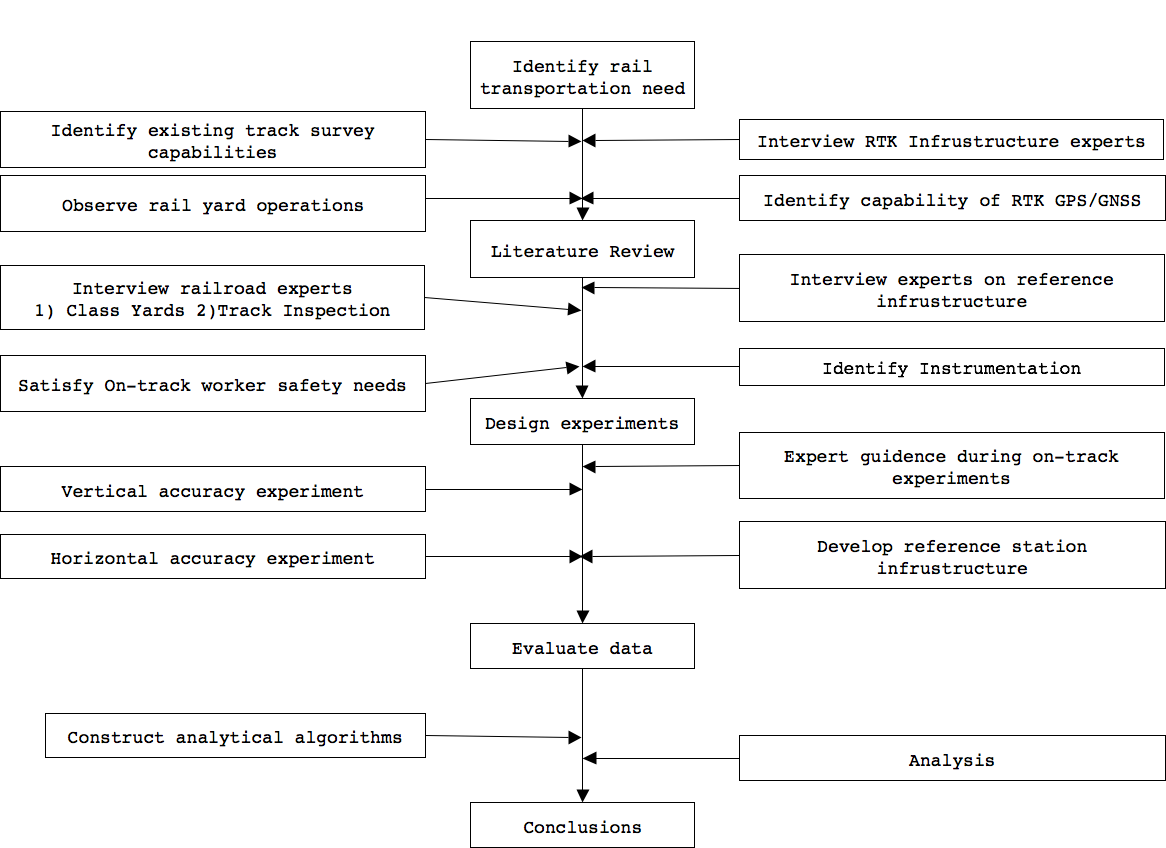
\includegraphics[width=6in]{graphics/research_plan.png}
	\caption{Research Plan}
	\label{fig:plan}
\end{figure}
The research investigated the capabilities of wireless measurement, in particular RTK GPS/GNSS, over active track. Due to federal and private property laws restricting access to active track, all research activities were performed adhering to the provisions of 49 CFR \S214 railroad workplace safety regulations, subpart C \textit{Roadway Worker Protection}~\citep{49CFR214300} and subpart D \textit{On Track Roadway Maintenance Machines and Hi-Rail Vehicles}~\citep{49CFR214500} as well as specific rail company rules and procedures set out by the employee in charge during job safety briefings. 

Track location of bowl tracks in a hump yard was determined from single epoch track observations from a GPS mounted on a locomotive traversing an active hump yard. The track positions were used to produce profiles for each bowl track in the yard. Relative vertical precision and base station observations were used to evaluate the yard environment for RTK GPS surveying by locomotive.

RTK augmented horizontal track measurements used single epoch RTK observations from an antenna mounted on the centerline of a track inspector's Hi-Rail. Mainline track alinement was evaluated by means of a software modeling the string lining method to determine the degree of curve from X, Y, Z track coordinates. Degree of curve ($D_c$) determined by the string line model was compared with $D_c$ determined by a track geometry car over an identical tangent segment.

An evaluation of RTK GNSS to determine track occupancy was made by multiple Hi-Rail traverses with RTK GNSS instruments across multiple parallel segments of mainline track. Positions observed over identical and parallel segments of tangent and circular track were evaluated for cross-track error\footnote{per Allen et al., \pageref{fig:trackRef}} for the likelihood of determining track occupancy by an RTK GNSS equipped mobile rail vehicle.

The electrical point of reference for a GPS/GNSS antenna is the phase center. The phase center is offset some distance from a physical reference location on the antenna housing. The physical antenna reference for each of these experiments was the mounting surface or antenna reference point (ARP). The survey controller contains a table of offset distances between phase center and ARP for the antennas used during each experiment. A procedure to align the ARP on the track vehicle to a selected railway reference location\footnote{i.e., Track centerline, left (port) gauge side or right (starboard) rail.} was performed as part of the mobile track vehicle setup.

Estimates for the relative horizontal and vertical precision\footnote{Relative errors are errors and precisions expressed for and between pairs of network adjusted control points.} are calculated by the \emph{Survey Controller} software in the Trimble TSC2 controller. \emph{Trimble Survey Controller} software uses a algorithm to compute vertical precision:
	\begin{equation}
Vertical Precision (m) = ErrorScale * VDOP * ScaleFactor
	\end{equation}
Where:\\
${ErrorScale = \frac{\sqrt{ErrorE + ErrorN + ErrorU}}{PDOP}}$\\
ErrorE = CovENU[x][x]\\
ErrorN = CovENU[y][y]\\
ErrorU = CovENU[z][z]\\

Where CovENU is the aposteriori covariance matrix of the RTK solution from the RTK engine in the GNSS receiver.\\
\emph{ScaleFactor} is either 1 or 1/3 depending on whether the RTK engine is giving \emph{Survey Controller} 1-sigma or 3-sigma precisions, which depends on the version of RTK engine. The \emph{Survey Controller} display shows 1-sigma precisions.~\citep{Trimble2009vprec}\\

The observation procedure for these experiments progress from setup of an ad hoc  reference station in the case of experiment 1, or accessing a VRS reference network as in experiments 2 and 3; establishing a means of communication between the reference station/VRS and the track vehicle; aligning the antenna with a track reference point; and configuring the mobile receiver onboard the track vehicle.

%Hump yard profile design
\subsection{Experiment One: Hump Yard Profile Survey} \label{ResDHmpYd}

Experiment one asked whether RTK augmented GPS mounted to a locomotive could measure the  vertical profile of bowl tracks in an automatic classification yard without the need for track closures.

The objective of experiment one was to use RTK GPS instrumentation mounted to a locomotive to survey an active hump yard in order to produce track profiles. The survey data was used to create information products which were handed off to the rail company sponsor in preparation for a yard-wide resurfacing project.
%{Ad Hoc Base Station Procedure}

The hump yard survey used a single RTK reference station transmitting correctors via UHF radio to a mobile receiver onboard a locomotive.  The ad hoc reference station components are listed in table \ref{tab:inst}. A fixed-height tripod at 1.5 meters supported the GPS and UHF antennas. The ad hoc reference station was set on top of a two story masonry structure to maximize height above average terrain (HAAT) for UHF data reception by the roving receiver aboard the locomotive as shown in figure figure \ref{fig:AhRS}. The elevated location provided sufficient HAAT to enable reception of correctors across the yard and to NGS benchmark EB1559 located 8,500 feet from the 25 watt UHF transmitter.

The autonomous horizontal position of the reference station (CP1) was adjusted by using the results of NGS OPUS from observations recorded during two sessions. The first session was 2008/05/26 14:21:00 to 21:44:00 UTC with the second session 2008/05/27 12:12:00 to 18:50:00 UTC\label{baseRefPeriod}. The compressed observation files were converted\footnote{Using Trimble \emph{runpkr00} under Unix.} to the Receiver INdependent EXchange (RINEX) format and submitted to the National Geodetic Survey Online Position User Service (NGS OPUS) for position determination. The autonomous horizontal position of the ad hoc reference station (CP1) was adjusted to the mean northing and easting of the two NGS OPUS reports exhibited in Appendix A, pages \pageref{opus1}~and~\pageref{opus2}.

The autonomous vertical position of the reference station was adjusted using RTK observations on a NGS benchmark, permanent identifier (PID) EB1559. The benchmark was located 8,508 from the ad hoc RTK reference station. The elevation of CP1 was adjusted to minimize the difference between the observed and the published NAVD88 elevation for the first order class II benchmark. The PID datasheet for EB1559 is exhibited in Appendix A, page \pageref{EB1559}.

Multipath concerns were examined at the reference stations by generating a full TEQC~\citep{EsteyTEQC} (Translation, Editing, and Quality Check) report from the reference station RINEX observation and navigation files. The TEQC report is exhibited in Appendix A.

% AhRS setup photo
\begin{figure}[!h]
\begin{center}
	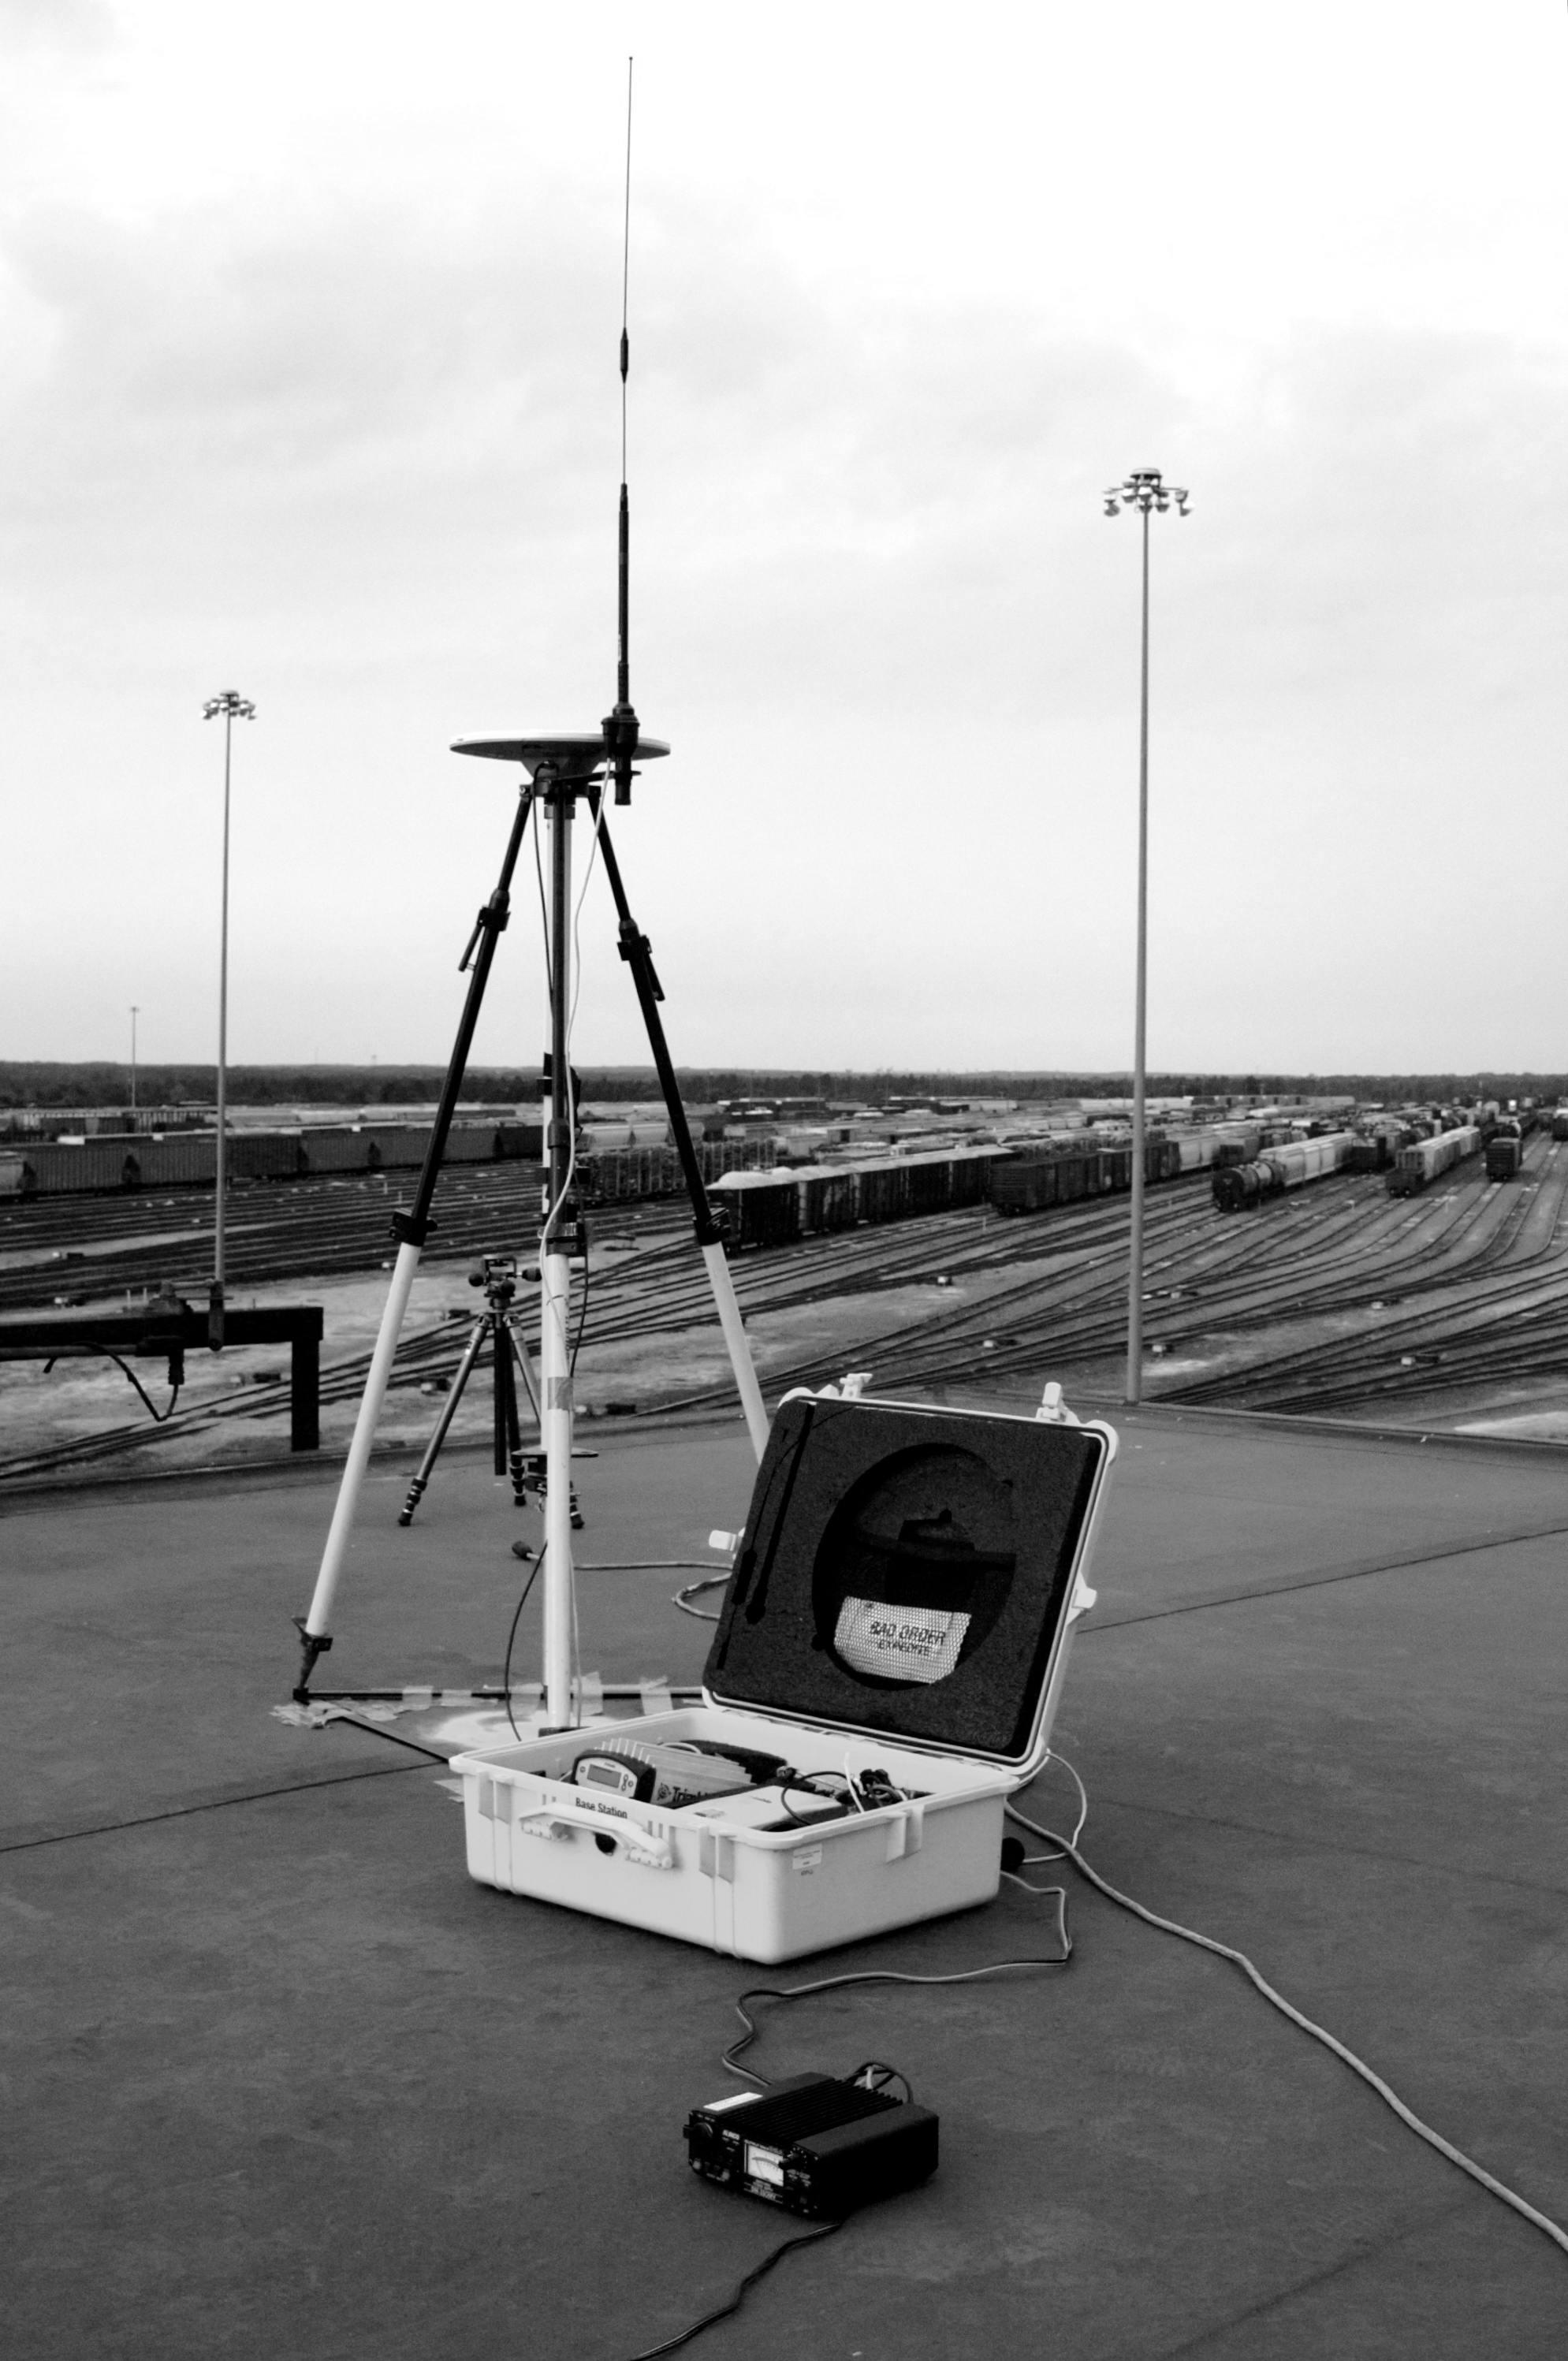
\includegraphics[scale=0.5]{graphics/AhRS_hamlet_BW}
	\caption{Ad hoc Reference Station}
	\label{fig:AhRS}
\end{center}
\end{figure}

An EMD SD60 yard locomotive was equipped with the mobile\#1 instrument indicated in table \ref{tab:inst}. The mobile GPS antenna mount was collocated with an omnidirectional UHF antenna and secured to a SECO magnetic base as illustrated in figure \ref{fig:locoAnt}. The antenna mount was fitted with a wire rope safety lead to secure the antenna assembly to a fixed member on the locomotive cab to prevented injury to locomotive operators or ground personnel in the event the antenna was dislodged by handling rail cars. 
% AhRS setup photo
\begin{figure}[h!]
  \begin{center}
    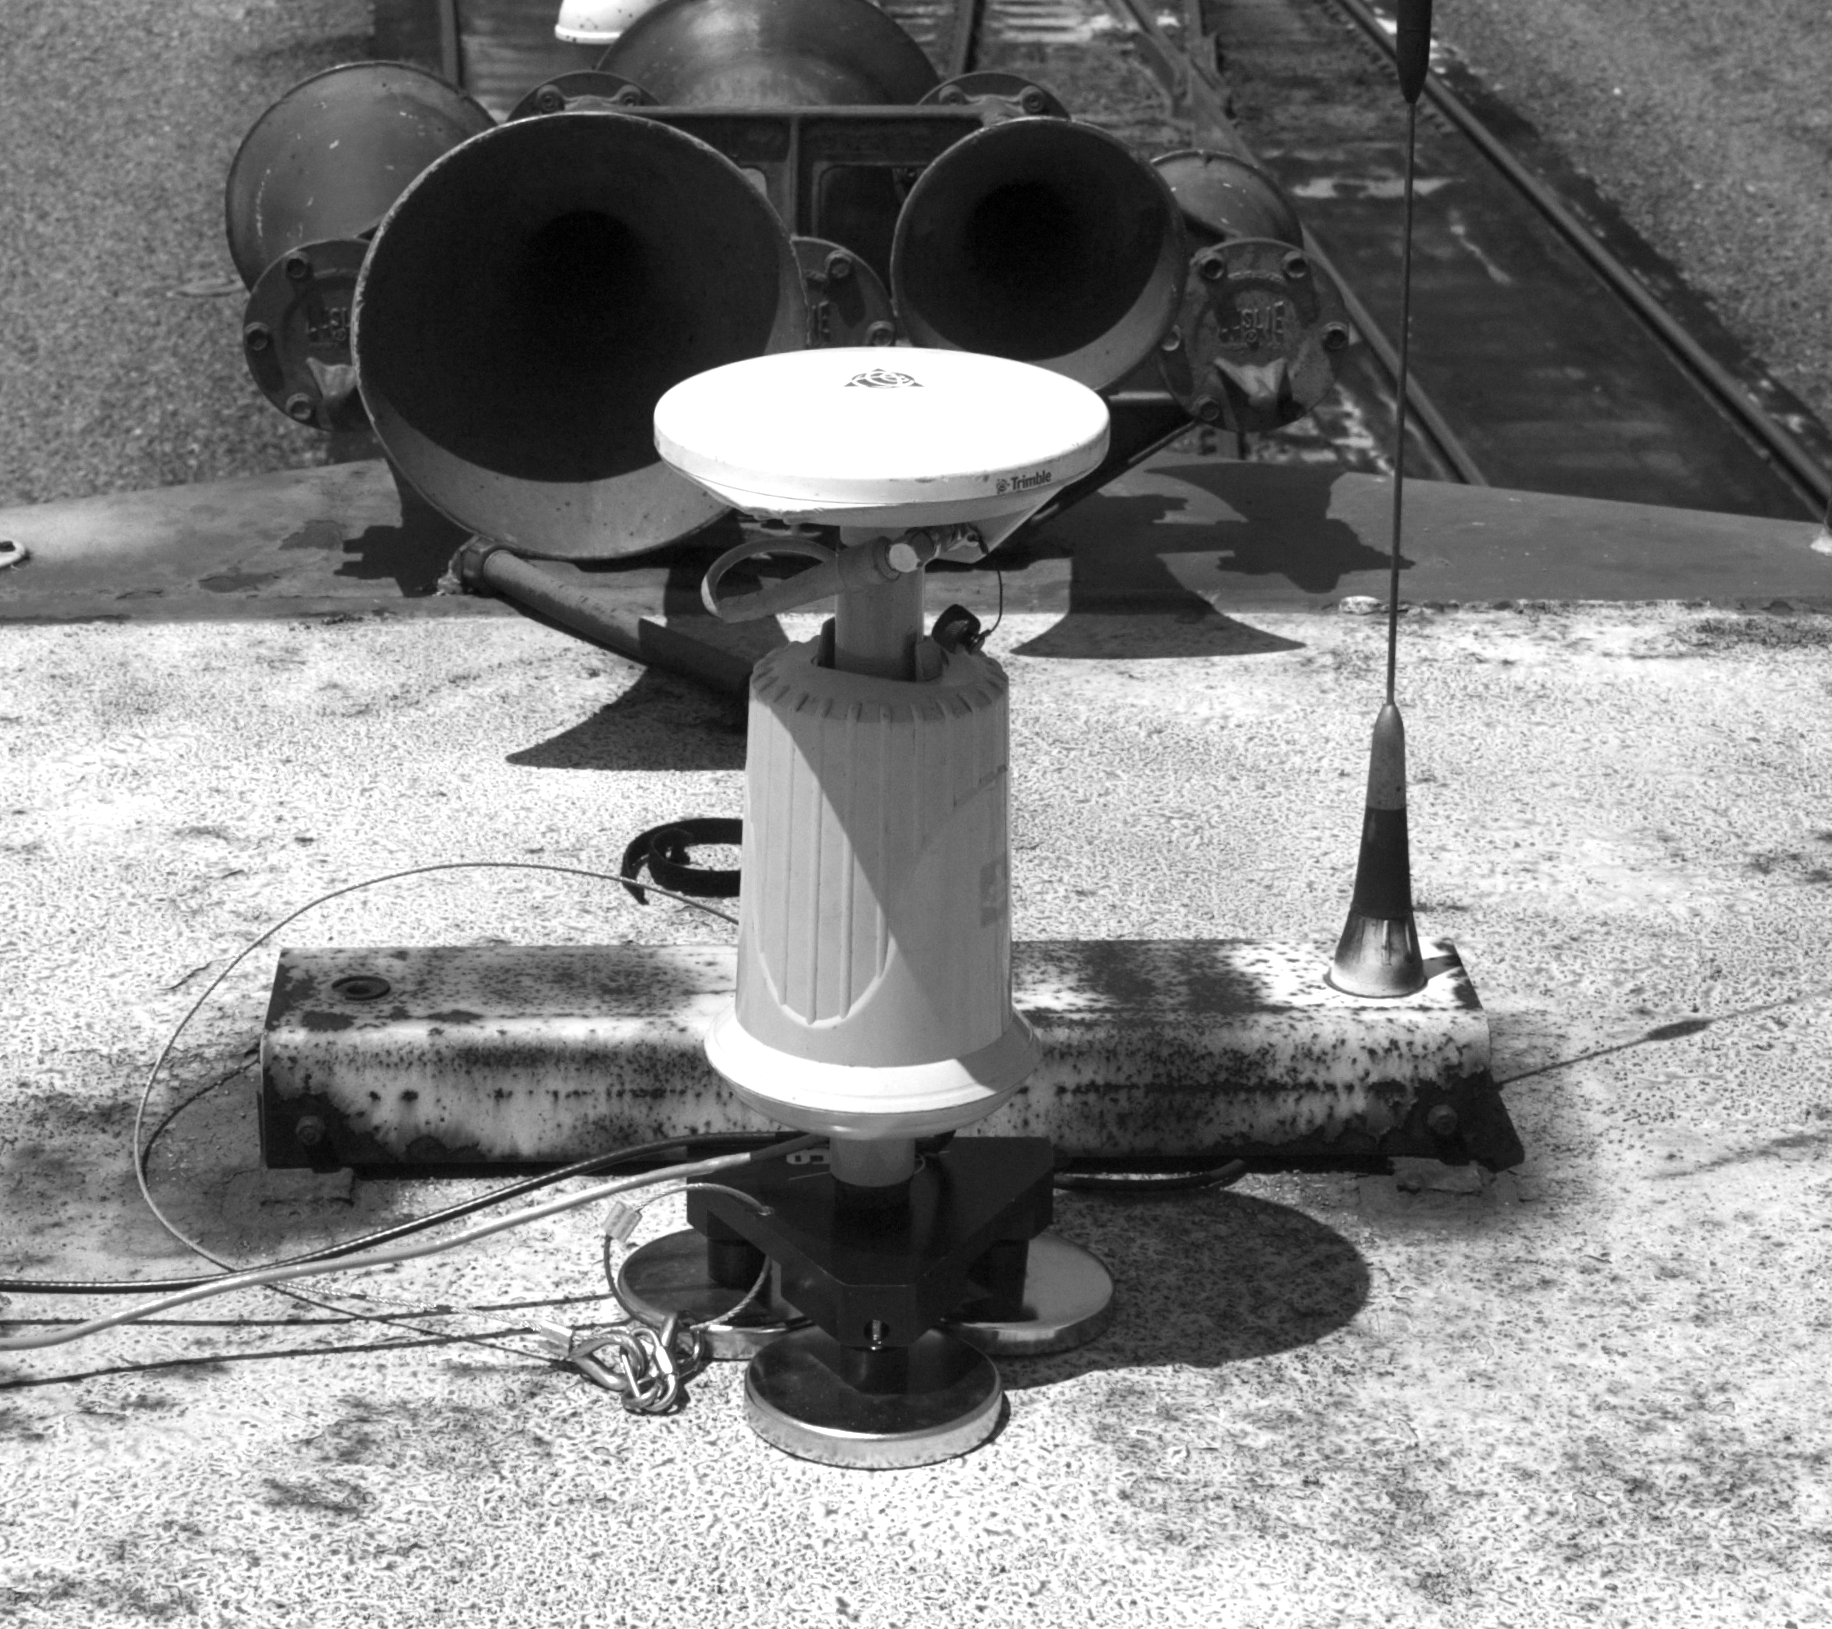
\includegraphics[width=0.48\textwidth]{graphics/AntennaMountBWcrop}
  \end{center}
  \caption{GPS/UHF Antenna Setup on Locomotive}
  \label{fig:locoAnt}

\end{figure}
The antenna was aligned with the track centerline in an area designated by the yardmaster and blue flagged during installation to insure the safety of research and railroad company personnel working around the locomotive. The generalized procedure for aligning a GPS/GNSS antenna mounted to a track vehicle with a horizontal track reference and determining the antenna reference point from the top-of-rail elevation is described following and referencing figure~\ref{fig:antAlign}.

% Antenna alignment procedure
\subsubsection{Antenna Alignment Procedure}
\label{Antenna Alignment}
\begin{enumerate}
\item A job safety briefing is conducted by the rail company employee-in-charge.
\item A frequency in the 450~Mhz band is selected by monitoring voice traffic on available channels, as data is a secondary use of this spectrum. The ad hoc reference station is programed with an autonomous position, and corrector transmission initiated.
\item  A section of tangent track approximately 300 feet long is blue flagged and made safe by setting a derail and locking out the track switch as discussed during the job safety briefing.
\item Track centerline points are measured on either end of the calibration area, figure~\ref{fig:antAlign} points A and A'. The centerline points are observed with a Trimble R8 instrument for 180 epochs.
\item A line feature representing the track centerline is created in the survey controller between points A and A'.
\item The center point of the line feature is determined. Two points, referenced in figure~\ref{fig:antAlign} as points B and B', are observed at the the top of each rail for 180 epochs.
\item A second line feature between points B and B' is created in the survey controller.
\item A point located by intersecting lines A-A' and B-B', figure~\ref{fig:antAlign} point C, is determined by the \emph{Survey Controller} software.
\item The mean elevation of the top of rail observations is calculated and assigned to point C.
\item The GPS/UHF antennas and magnetic base mount are placed in the approximate center of the top of the locomotive cab. A wire rope safety harness connecting the antenna mount to the locomotive horn or other suitable anchor point is secured.
\item The survey controller is connected to the GPS receiver in the track vehicle. The previously created data file with the alignment features described above is opened.
\item Blue flags are removed from the locomotive by the persons that placed them. Derails are stowed and facing point track switch operators are unlocked. Movement authority is obtained from the yardmaster by the locomotive engineer.
\item The locomotive is moved to locate the GPS/UHF antenna mount over point C.
\item The locomotive is secured and the antenna mount moved in small increments to intersect the centerline by observing the instantaneous antenna location in the map view of the controller. A period of  ten seconds between movements is allowed for the position to settle in the map display.
\item The survey controller antenna height is set to zero. Figure~\ref{fig:antAlign} point D is observed for 180-epochs. An inverse calculation is performed between points C and D. The elevation difference is recorded as the antenna height.
\item A survey style is created in the \emph{Survey Controller} software containing the antenna height above the top-of-rail elevation. Due to variation in cab height above top-of-rail, the survey style is named for the particular locomotive unit number used in the antenna alignment. Likewise for individual Hi-Rail vehicles.
\end{enumerate}

% Alinement drawing
\begin{figure}[h!]
  \begin{center}
    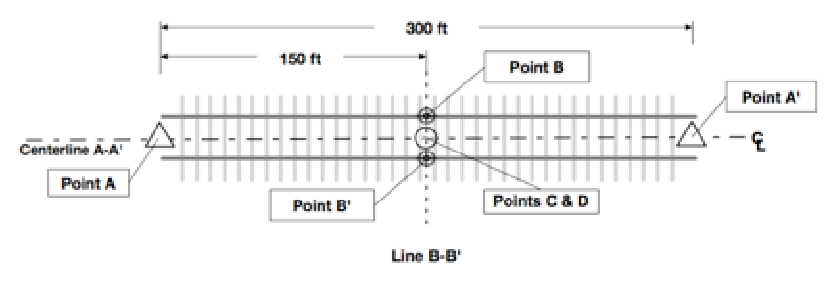
\includegraphics[scale=0.40]{graphics/antennaAlinement.png}
  \end{center}
  \caption{Track Vehicle Antenna Alinement Procedure}
  \label{fig:antAlign}
\vspace{-20pt}
\end{figure}

RTK correctors were broadcast from the single reference station by UHF data radio and used to augment the GPS receiver aboard the locomotive. A survey controller connected to the receiver managed and automated data collection by recording single epoch observations with a nominal horizontal separation of ten feet. Track profiles originated at a common reference point at the hump end of the bowl and terminated at the pullout-end switch for each track.

The pullout end of the bowl was surveyed first, from pullout switch to foul point\footnote{The track foul point is the demarcation between hump and pullout end movement authority. CSX standard is a 7-11 rule; which defines the foul point to be determined 11 feet beyond the point where the field side rails of adjacent track are 7 feet apart.~\citep{vanWormer07}}. The hump end of the bowl was surveyed during a shift change, from the hump to foul point, to minimize disruption to humping operations. Locomotive movement across the pullout end of the yard was coordinated between the locomotive operator and pullout end humpmaster\footnote{Responsible for outgoing train makeup and movement.}. Track traverses began at the pullout end switch and progressed to the foul point. The automatic numeric sequencing of the survey controller was used to produce unique point identifiers. The controller sequence was constructed by concatenating: 1) the  two digit track number; 2) a single digit traverse counter; 3) a three digit point sequence beginning at 000 and incremented by one at each observation in sequence. Points recorded onboard the locomotive were feature coded as centerlines.

The hump end survey was performed in coordination with the hump end humpmaster\footnote{Responsible for railcar sequencing and switching into the bowl.} during the yard shift change to minimize the impact of the survey interrupting yard production. The locomotive traverse of the hump end began at the hump, through the retarder and track leads, finishing at the track foul point. The unique point identification scheme previously described was not performed due to time constraints. The hump, leads, and track points were separated post survey.

Points of interest (POI) were surveyed on the ground with the static module referenced in table \ref{tab:inst}. The static receiver was mounted to a 2 meter range pole. Multiple epoch observations (3-6) were recorded at each point of interest. Feature codes distinguished switch points, wheel detectors, retarder inlet/outlet, and foul points. Switch points and retarders were identified by rail company reference number. Wheel detectors were identified by track and sequence number. Ground point safety was superintended by a rail company employee.

% Hump Yard Data
\emph{Variables of analysis}: The mobile instrument \#1, table \ref{tab:inst} produced these variables:
\begin{description}	
	\item [Horizontal coordinates]: US State Plane, North Carolina 3200,US survey feet.
	\item [Vertical datum]: NAVD 88, height above ellipsoid 2003, in US survey feet.
	\item [Estimated Vertical Precision]: Determined by \emph{Survey Controller} software, US survey feet.
	\item [Time \& Date]: Local, EST of observation.
	\item [Count]: SVs in view of the mobile\#1 GPS antenna.
	\item [Vertical Dilution of Precision]: VDOP, A unit-less figure of merit expressing the relationship between error in in user position, and the error in satellite position.
\end{description}

Yard observations were exported from the \emph{Survey Controller} software and separated into layers organized by lead, group, and track. Deconstructing the aggregate observations enabled individual tracks to be configured as a continuous series of points by activating the particular layers in TGO.

\begin{itemize}
	\item Hump lead
	\item Main retarder
	\item Intermediate retarders
	\item Group retarders
	\item Group leads
	\item Bowl tracks
\end{itemize}

A properly configured track was apparent as a continuous series of points extending from the hump through the desired track to the pullout end switch.

Locations of track POI (i.e., track switch points, retarder inlet and outlet, wheel detectors) were associated with a position nearest a particular rail. The POI was observed at the center top-of-rail nearest the POI physical location using the static survey instrument. The position of each POI was adjusted post survey to be coincident with the track centerline.

Continuous track observation names were renumbered in the TGO software, in series progressing from hump to pull out. Feature codes enabled separation by feature. The \emph{TGO} software was used to create line work by connecting consecutive centerline points. The line work and observation data were exported from TGO in the ESRI\footnote{Environmental Systems Research Institute, Inc.} shapefile format. The point data was also exported as a comma delimited (CSV) format and imported to a \emph{Google Docs} spreadsheet. A linear reference was determined for each point according to equation \ref{eq:horzSta}. Elevations and linear references were scaled and input as an overlay to a CAD drawing containing the track design grade\footnote{Provided by the rail company sponsor.}. 

Each track profile was plotted as an overlay to the provided CAD drawing. The design profile in the CAD drawing is relevant to the rail company in a making a volumetric assessment of surfacing material required to bring the relief of each track into vertical alignment with the design grade. Calculation of surfacing material quantity is outside the scope of the experiment. The design grade and locomotive survey result will be used as a comparative tool, limited to providing track profile deviation from design grade.

The shapefiles will be added to ESRI ArcMap software where a plan view of of the bowl area track elevation and vertical precision estimate will be represented in plan view. The vertical precision map will show lower quality vertical precision for points > 0.1 feet in a contrasting color to those of greater precision. The plot will be examined for the distribution of lower quality data patterns.

Acceptable elevation quality will be apparent as a smooth track profile. Poor quality observations will appear with greater variation between points, resulting in a jagged or sawtooth profile. Poor quality elevations will be identified and correlated with: observation time; vertical precision estimated by the receiver; and reference station observations during the period.

The vertical precision calculated by the \emph{Survey Controller} software was used to determine descriptive statistics and to plot a histogram for analyzing the quality of GPS observations by the mobile instruments.

%Horizontal stationing equation
	\begin{equation}
	{sta_k} = {match~point~offset} + {\sum_{k=2}^n}  {\sqrt{(x_k - x_{k-1})^2 +( y_k - y_{k-1})^2}}
	\label{eq:horzSta}
	\end{equation}
\begin{quotation}
Where \emph{k} =  a point in the ordered sequence of observations, and \emph{n} = the number of observations in the track segment, and the match point offset is the horizontal distance from the top of the hump to switch point 1574.
\end{quotation}

Experiment one:
\begin{enumerate}
	\item Produced an alignment procedure for alignment of the GPS antenna with the centerline top-of-rail location.
	\item  Collected continuous single epoch observations on a nominal 10 foot horizontal spacing with RTK augmented GPS onboard a locomotive in an active hump yard. 
	\item Resulted in the production of a plan-view color-map of track elevation for the bowl area of a hump yard.
	\item Resulted in the production of a plan-view color-map of relative vertical precision as determined by the \emph{Survey Controller} software for points measured in the bowl area of the yard.
	\item Resulted in the production of a two-dimensional profile drawings for each track in 1:1 and 1:5 vertical scale.
	\item Determined the descriptive statistics of the relative vertical precision as determined by the \emph{Survey Controller} software for the locomotive mounted GPS .
	\item Resulted in the production of TEQC reports for two ad hoc reference station observation sessions.
\end{enumerate}

% Mainline Track alinement design
\subsection{Experiment Two: Determining Horizontal Track Alinement}
\label{Ex2Design}
This research asks whether RTK augmented GPS and GNSS instruments mounted to a common track vehicle can determine horizontal track alinement comparable those achieved by specialized track geometry vehicles. The objective of the experiment was to perform multiple mainline track surveys with RTK instruments mounted to a Hi-Rail vehicle; the development and demonstration of a software model using the string lining procedure in order to produce horizontal track alinement. The track alinement survey employed a series of CORS RTK reference stations along the survey route, networked to the Ohio Department of Transportation, Aerial Mapping Virtual Reference Station (ODOT VRS) server.

The ODOT VRS was used to minimize the $\pm$1 ppm error incurred as distance increases from a reference station. The VRS creates a new virtual reference station when the baseline between the track vehicle and the previous VRS created reference station increased beyond a distance programmed in the VRS. A public cellular data service was used to exchange security credentials with  the ODOT VRS server, receive correctors, and apply them to a mobile receiver onboard a track inspector's Hi-Rail. A survey controller connected to the mobile receiver recorded single epoch observations with a nominal horizontal point separation of five feet with mobile instrument\#2 (table \ref{tab:inst}) and ten feet with mobile instrument\#1. Nominal point separation was based on the receiver processing speed for Hi-Rail traverses in the range of 10 to 30 mph.

% Alinement Study Area
Two mainline track segments of different character were traversed during this experiment. The first segment can be characterized as multiple parallel track, signalized, Class 4, with a maximum allowable track speed between 30 and 50 mph, carrying a freight volume of 25 to 35 MGT/yr\footnote{Million Gross Tons per year}. This segment is referenced as C\&O Kanawha subdivision, from mile post 494 to 523 (MP494-523). Continuous observations over this segment demonstrates the capability of an RTK VRS over a wide area.

A second segment, characterized as single track, dark territory, Class 3, with allowable track speed between 10-30 mph, carrying a freight volume of less than 10 MGT/yr, is referenced as C\&O Ohio River subdivision from mile post 210 to 207 (MP210-207). This segment was selected for study as the segment had been examined previously by Szwilski~\citep{Szwilski03}. Additionally, data was made available from CSX's Gauge Restraint Measurement System\footnote{A specialized, self-propelled, track geometry car.} (GMRS) across this segment. Degree of curvature (${D_c}$) from the GMRS was compared with the horizontal alinement model by selecting a tangent segment for comparision. An ideal measurement across a tangent segment would result in a ${D_c}$ of zero. Therefore, the ${D_c}$ deviation from zero across the tangent segment was used to compare the GMRS measurement with RTK modeled ${D_c}$ measurements.

% FRA alinement figure
\begin{figure}[!htp]
	\vspace{-20pt}
		\begin{center}
			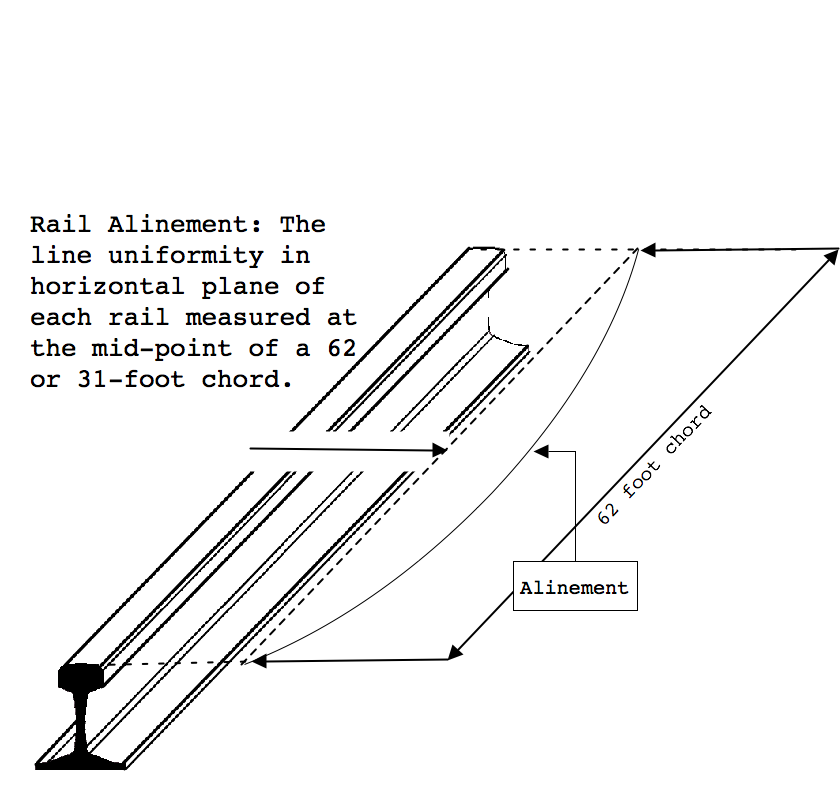
\includegraphics[width=3in]{graphics/HorzAlignment.png}
			\caption{Horizontal Alinement}\label{fig:Alinement}
		\end{center}
%	\vspace{-30pt}
\end{figure}

The track observations were used as inputs to a software to determine the ${D_c}$ modeling the FRA guidance manual instructions for using the string line method.
Experiment two objectives sought to:
\begin{enumerate}
	\item Collect continuous single epoch observations with RTK augmented GPS/GNSS mounted to a track inspector's Hi-Rail over at least 29 continuous miles of mainline track. Point spacing was a nominal 10 foot for mobile configuration\#1 and 5 foot horizontal spacing for mobile configuration \#2 (see table \ref{tab:inst}).
	\item Develop a software model for calculating degree of curvature (${D_c}$) from X, Y, and Z coordinates obtained from track vehicle observations. The software model replicated the string lining method described in FRA \emph{Track Safety Standards Compliance Manual}~\citep[pp.26-30]{2007FRATrack} using a 62 foot chord length and 15.5 foot stations.
	\item Compare two methods of measuring ${D_c}$ over tangent track. The first method utilized data from a specialized track geometry car, CSX's GMRS. The self propelled GMRS is designed specifically for the purpose of obtaining ${D_c}$ (and other track alinement parameters\footnote{Gage, crosslevel, profile, ${D_c}$}) from the string lining method. The second method utilized data obtained from an RTK GNSS instrument mounted to a track inspector's Hi-Rail and a software to model the string line method from the Hi-Rail data.
	A traverse of identical tangent track segments was compared for cross-track\footnote{See Allen, et al., figure \ref{fig:trackRef}, page \pageref{fig:trackRef}} centerline deviation using descriptive statistics. Identical segments were determined by selecting beginning and ending mile post reference locations.
	\item The ${D_c}$ was determined and track elevation measured using RTK survey equipment mounted to a track inspector's Hi-Rail across a continuous 29 mile track segment. The modeled ${D_c}$ was compared with company supplied track charts to correlate the location and magnitude of curves. Structures responsible for loss of signal (LOS) were identified.
\end{enumerate}

\emph{Variables of analysis}: The mobile instrument \#1 and \#2, table \ref{tab:inst} produced these variables:
\begin{description}
	\item [Horizontal coordinates]: UTM, Zone 17 North, US survey feet.
	\item [Vertical datum]: NAVD 88, height above ellipsoid 2003, US survey feet.
	\item [Time \& Date]: Local, EST.
\end{description}
\emph{Variables of analysis}: The CSX GMRS produced these variables of analysis:
\begin{description}
	\item [MP]: Mile post offset distance, decimal miles.
	\item [${D_c}$]: Degree of curve, 62 foot chord.
\end{description}

%Data Collection Experiment 2

The mobile antenna (table \ref{tab:inst} mobile~\#2) was alined using the generalized procedure listed on page \pageref{Antenna Alignment}, and mounted to a track inspector's Hi-Rail vehicle as illustrated in figure \ref{fig:antHi-Rail}. The receiver was programmed to process observations in ``low latency'' mode, which uses approximately 20 milliseconds to compute each observation, degrading the manufacture's stated horizontal accuracy of $\pm$~1~cm by an additional centimeter~\cite[pp.8]{Trimble5700}~\cite[pp.9]{TrimbleR7gnss}.

% Hi-Rail antenna
\begin{figure}[h!]
  \begin{center}
    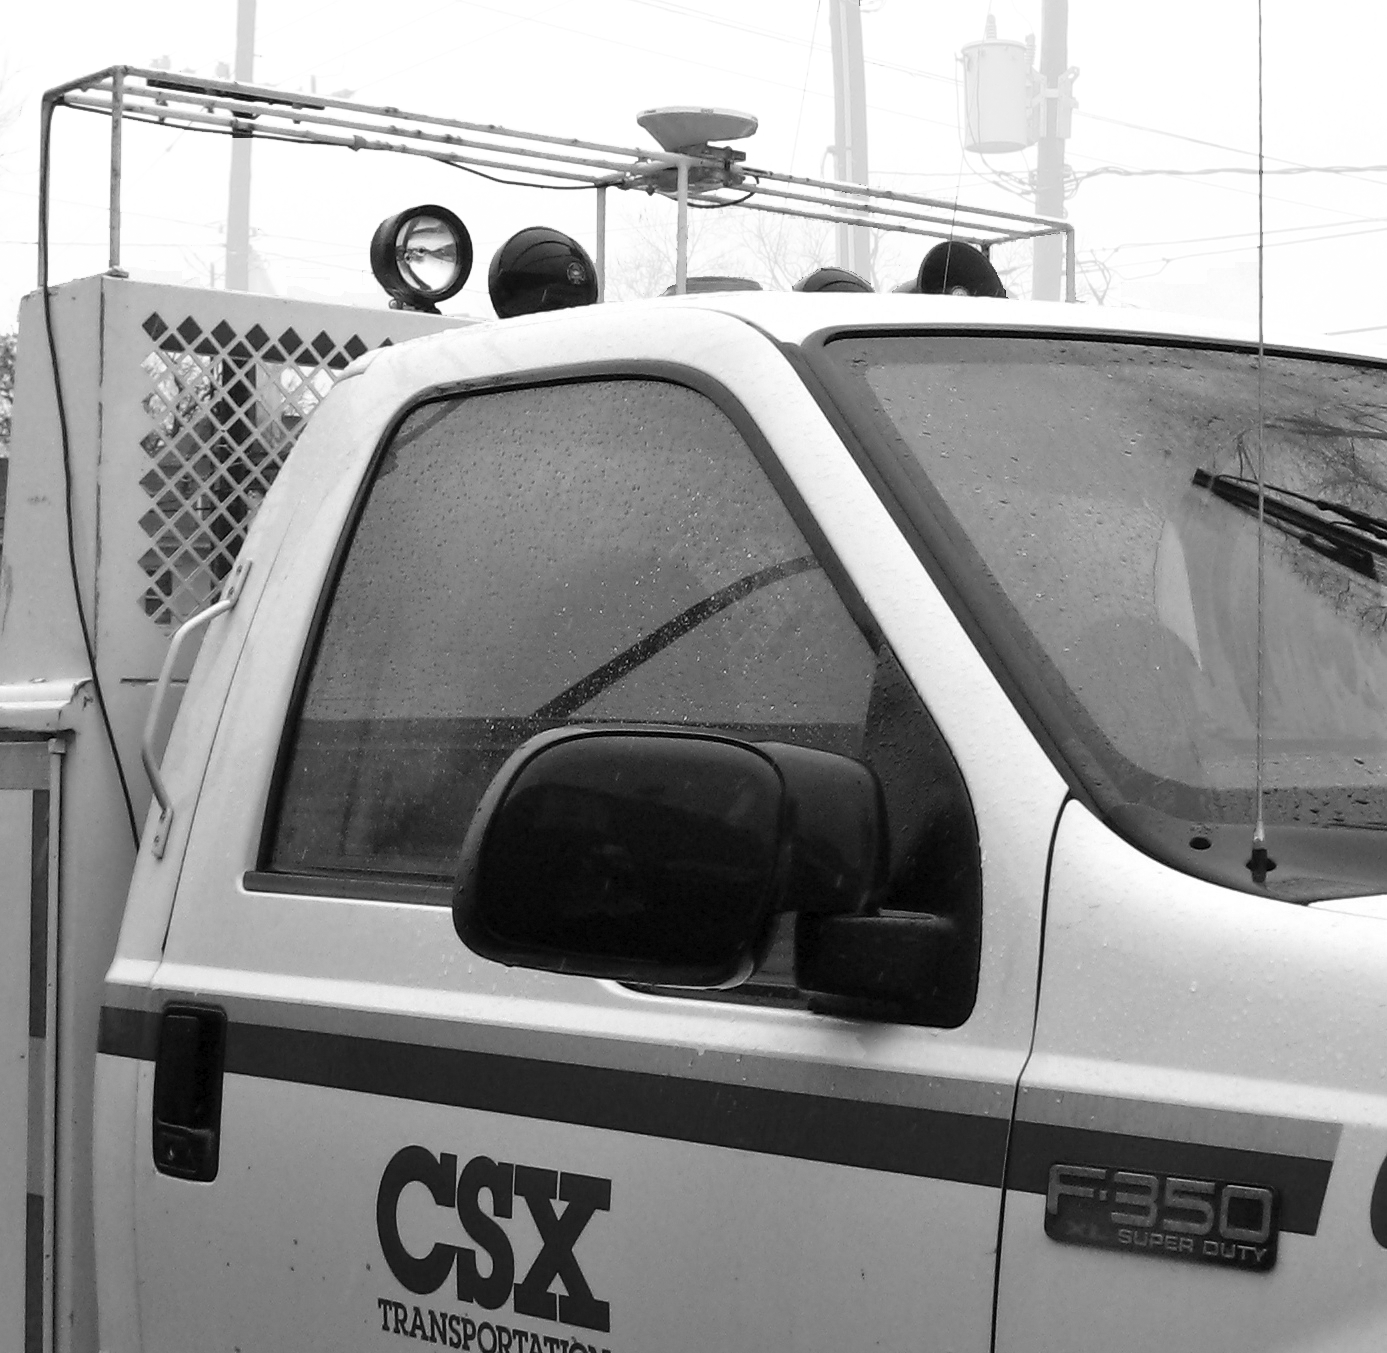
\includegraphics[scale=0.50]{graphics/HiRailAnt_modBW.png}
  \end{center}
  \caption{GNSS Antenna Mount, Hi-Rail}
  \label{fig:antHi-Rail}
\vspace{-20pt}
\end{figure}

The controller was programmed to collect observations on a nominal 5 foot spacing. Mile post centerline locations were determined during a traverse of the research area. Mile post centerline locations were determined by positioning the Hi-Rail perpendicular with a mile post and observing the location for five seconds, resulting in 3 to 6 epoch observations.

The observations recorded by survey controller were transferred to \emph{Trimble Geomatic Office} (TGO) software. Observations were separated into centerline and mile post layers, then exported in an ASCII comma delimited text format that included observation ID, feature code\footnote{centerline, mile post}, northing, easting, elevation, time and date, and number of observed SVs.

Mainline track locations are reported as a linear reference from a wayside mile post monument. A track reference reports the mile post number plus the offset from the monument in decimal miles. Mile post references are typically measured by odometer, therefore the offset distance from a mile post is the accumulated slope distance. An additional novelty of mile post distances in the United States is the inconsistent measure between reference marks. To determine a mile post reference location, the accumulated slope distance between observations from a mile post to the location of interest is divided by the distance between mile posts in feet, then added to or subtracted from the mile post number depending on the direction of travel\footnote{Milepost offset is added to the mile post when the direction of travel is with increasing mile post numbers, offset is subtracted with decreasing mile post numbers.}. The calculation is illustrated in equation \ref{eq:accumSlopeD}.

% Track Alinement Analysis

Track position variables processed by the model to determined the degree of curve (${D_c}$), following the string lining method described in FRA \emph{Track Safety Standards Compliance Manual for Track Classes 1-5} per 49CFR\S213.55~\citep{2007FRATrack}.

% Mile post reference equation
\begin{equation}
	MP_{k} =  MP_{num} \pm \frac{\displaystyle {\sum_{k=1}^n {\sqrt{(x_k - x_{k-1})^2 +( y_k - y_{k-1})^2 +( z_k - z_{k-1})^2}}}}{\displaystyle{\sum_1 ^n \sqrt{\Delta x_n^2 + \Delta y_n^2 + \Delta z_n^2}}}
	\label{eq:accumSlopeD}
\end{equation}
\begin{flushright}
Where \emph{n} = the total number of observations between mile monuments.
\end{flushright}

The string lining method as practiced by track inspectors and superintendents as described in the FRA \emph{Track Safety Compliance Manual} determines points of greatest alinement deviation by moving a 62 foot string along the track in increments until the point with maximum deviation is found. The software model uses a similar approach, incrementally moving a chord along lines connecting an ordered series of RTK track observations. The distance from a chord's middle ordinate to a line segment  determines the mid-chord offset (MCO). The software model determination of MCO from RTK observations as represented by figure~\ref{fig:strLine}.

End point coordinates for a 62 foot chord are determined by extending a 62 foot radius circle originating from the beginning station coordinate, represented by figure~\ref{fig:strLine} station~($x_o, y_o$) and intersection a line segment defined by:
\begin{itemize}
	\item An endpoint defined by the farthest point from the chord circle origin inside the chord circle.
	\item An end point defined by the the nearest point outside the circle.
\end{itemize}

The intersection is indicated at point ($x_{int}, y_{int}$) in figure~\ref{fig:strLine}, lying between points D and E.

% String Line Illustration
\begin{figure}[!htp]
	\begin{center}
		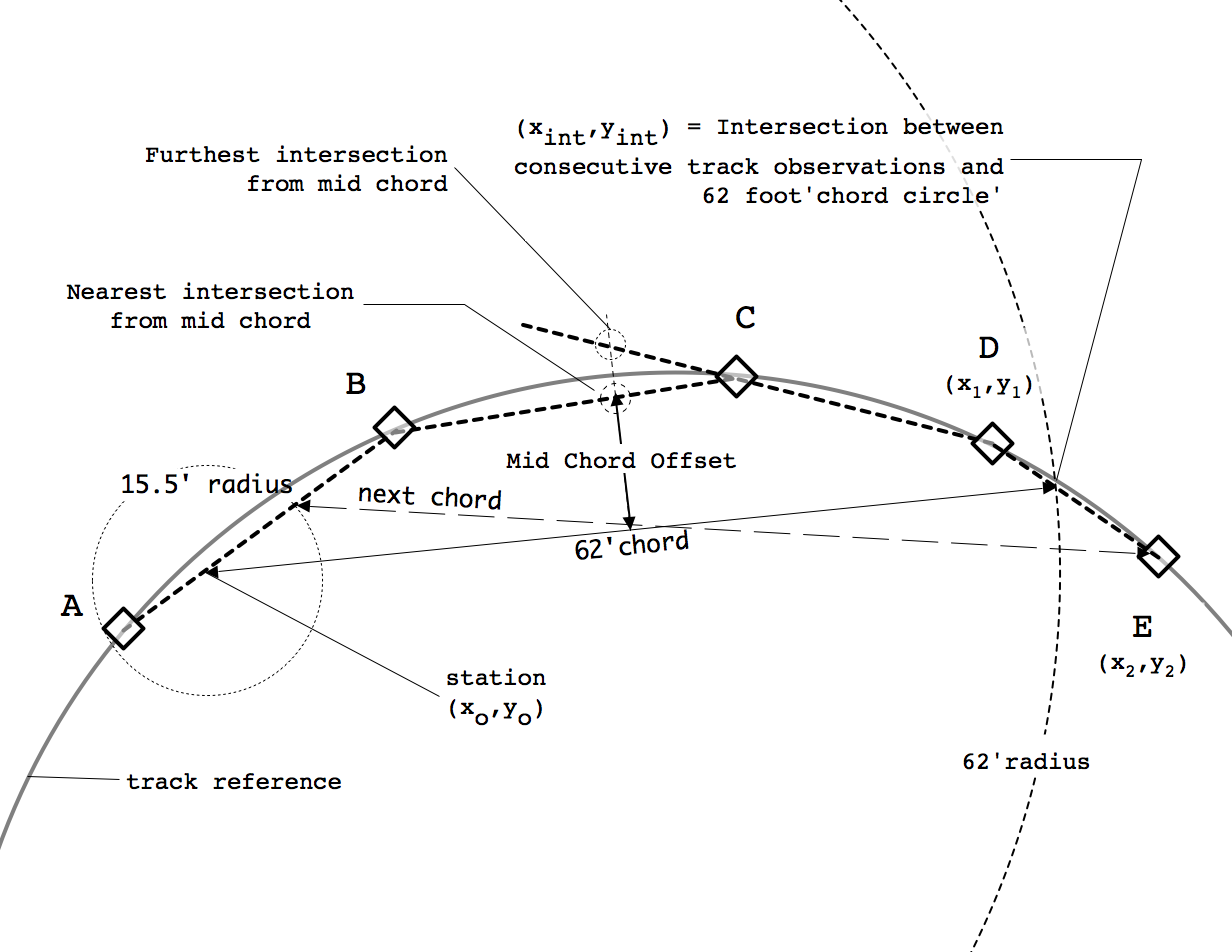
\includegraphics[width=13cm]{graphics/stringLining.png}
		\caption{Modeling the String Line Method from RTK Track Observations}
		\label{fig:strLine}
	\end{center}
\end{figure}

The MCO is determined from an line orthogonal with the mid point of the chord, and the mean of the intersection with the nearest and farthest of two lines projected from the three observations nearest to the middle ordinate (figure~\ref{fig:strLine} points B, C, and D). The distance from the chord mid point and the mean intersection determines the MCO. The degree of curve (chord definition) is then found from the MCO and chord length in feet by the relationship~\citep{1964hickerson}.
	\begin{equation}
		D_c = \frac{45840 \times MCO}{chord^2}
		\label{eqn:degOcrv}
	\end{equation}
	
The model assigns a mile post reference to $D_c$ using the location of the mean intersection and equation \ref{eq:accumSlopeD}.

The coordinates of the next station are found by intersecting the stationing distance in a similar fashion to the chord circle intersection. Figure~\ref{fig:strLine} illustrates determination of a 15.5 foot station. 

A railway can be described as a smooth, continuous shape. As an aid to exploring the $D_c$, a smoothing algorithm is applied to the $D_c$ verses mile post reference.  The \emph{rlowess}\footnote{The \emph{rlowess} method is a local regression using weighted linear least squares and a 1st degree polynomial model that assigns lower weight to outliers in the regression. The method assigns zero weight to data outside six mean absolute deviations~\citep{matlab09}.} method of the \emph{smooth} function in the Matlab \emph{Curve Fitting Toolbox}$^{TM}$ was selected as a data exploration tool.

Experiment two:
\begin{itemize}
	\item Compared RTK observations by Hi-Rail with company track charts. The comparison between the model and track charts was examined to verify curve location, magnitude, and location of infrastructure affecting SV reception. Mile length was compared to the published track chart length.
	\item Determined descriptive statistics for  $D_c$  across a tangent segment for a geometry car and a RTK equipped Hi-Rail.
	\item Constructed a graphic solution for comparing $D_c$ measured by geometry car and RTK equipped Hi-Rail by plotting $D_c$ vs. mile post reference concurrently.
	\item Determined the variability between $D_c$ measured by geometry car and RTK equipped Hi-Rail across tangent track.
\end{itemize}

% Track Occupancy Design
\subsection{Experiment Three: Determining Track Occupancy} 
This experiment asked whether a common track vehicle using RTK augmented GPS/GNSS was able determine track occupancy by obtaining position accuracy defined by the FRA for a location determination system. The FRA LDS requirement stated in \emph{Differential GPS: An Aid To Positive Train Control}~\citep{1995FRADiffe} page 6, establishes the criteria to\\
\begin{quotation}
``...determine which of two tracks a given train is occupying with a very high degree of assurance (an assurance that must be greater than 0.99999 or (0.9$_5$)). The minimum center-to-center spacing of parallel tracks is 11.5 feet...''~\citep{1995FRADiffe}\\
\end{quotation}
The FRA specification is interpreted here to mean an observation must have a cross-track error no greater than $\pm \frac{11.5}{2}$ feet within a confidence interval 100*(1-${\alpha}$)\%, with ${\alpha}$~=~0.00001 or 99.999\%.

% Variables
\emph{Variables of analysis}: The mobile instrument \#2, table \ref{tab:inst} produced these variables:
\begin{description}
	\item [Horizontal coordinates]: UTM, Zone 17 North, US survey feet.
	\item [Time \& Date]: Local, EST.
\end{description}

Several traverses of a parallel multitrack segment were made by RTK GNSS equipped Hi-Rail. A track segment was selected based on the length of the tangent or curve and existence of adjacent parallel track traverses. The first traverse was designated as a reference centerline, and the centerline coefficients for tangent track determined by regression using the Matlab function \emph{regress}, taking the general form:

\begin{equation}
\label{tanReg}
[b,bint,r,rint,stats] = regress ( y, X)
\end{equation}

\emph{where};

\emph{y} is a \emph{n by 1} vector of observed Northings for each of n observations.

\emph{X} is a \emph{n by 2} matrix of observed Northings of the form ${[Northing,~1]}$ for each of n observations.\\

The function output \emph{b} containes the coefficient estimates, and \emph{bint} contains the upper and lower confidence bounds of the coefficient estimates. The residuals \emph{r} and residual intervals \emph{rint} that have no meaning in the analysis as physically, the residuals represent the distance from the track centerline to the observation along the Northing axis. The statistics in \emph{stats} contain the ${R^2}$ statistic, the ${F}$ statistic and its p-value, and an estimate of the error variance.

The slope is converted to an azimuth and back bearing by the function \emph{slope2Az}, listed in Appendix B. The azimuth of the tangent was verified by means of a graphical solution in \emph{TGO} software.

The cross-track\footnote{See Allen, et al, Figure \ref{fig:trackRef}, page \pageref{fig:trackRef}} distance between subsequent observations and the baseline was determined by the Matlab function \emph{perpDist2line}, code listing Appendix B, page \pageref{software}. The function equation \ref{tanXtrack} determines the cross-track distance from a reference tangent and an X, Y coordinate pair obtained from a subsequent track traverse.
%d = abs[(aX + bY +c)/srt(a^2 + b^2)]
\begin{equation}
d_{xt} = \left|\frac{ax + by + c}{\sqrt{a^2 + b^2}}\right|
\label{tanXtrack}
\end{equation}

\emph{where};

\emph{a, b, c} are the reference tangent centerline coefficients.

\emph{x, y} are the Easting and Northing coordinates of the observations.\\

For the circular curve case, the coefficients of the centerline reference origin and radius are determined from Northing and Easting observations using Matlab function \emph{regress}. \emph{Regress}. For the circular curve case, the function takes the general form:
\begin{equation}
\label{crvReg}
[b,bint,r,rint,stats] = regress ( y, X )
\end{equation}

\emph{where};

\emph{y} is an \emph{n~by~1} matrix of observed Northings and Eastings of the form ${[Easting^2+Northing^2]}$ for each of n observations.

\emph{X} is an \emph{n~by~3} matrix of observed Northings of the form ${[2*Easting,~2*Northing,~-1]}$ for each of n observations.

%crvAX = [crvA.easting*.2 crvA.northing*.2 numel(crv2.northing)*.-1]
%crvAY = [crvA.easting.^2 crvA.northing.^2]

The cross-track distance ($d_{xt}$) is determined from the difference between the circular curve radius and coordinate distance to the origin of the curve:
\begin{equation}
\label{crvXtrack}
d_{xt} = r - \sqrt{( x_p - X_o )^2 + (y_p - Y_o)}
\end{equation}

% Hypothesis test
The null hypothesis statement is the reference track is occupied if the distance between an RTK GNSS observation and the reference centerline is less than or equal to $\frac{11.5}{2}$ feet at a confidence of 100(1-${\alpha}$)\%. The Matlab function \emph{ztest}  was used for the z-test of the null hypothesis. The function output indicates whether the null hypothesis is a random sample from a normal distribution with mean cross track distance ($\mu_{d}$) less than 5.75 feet and standard deviation $\sigma$ of the reference tangent distances, against the alternative that the mean is not less than 5.75 feet. The result of the test indicates a rejection of the null hypothesis at the 100*(1 - 0.00001)\% significance level.

\begin{equation}
	h_{0}: \mu_{xt} < \frac{11.5}{2}
\end{equation}
\begin{equation}
	h_{1}: \mu_{xt} \ge \frac{11.5}{2}
\end{equation}

The null hypothesis asserts that the cross-track error population parameter is equal to or less than half the FRA guideline for minimum centerline-to-centerline track spacing. Rejection of the null hypothesis indicates insufficient statistical evidence exists to assert same track occupancy to the confidence interval suggested by the FRA~\citep[pp. 6]{1995FRADiffe}. 

The Z-test hypothesis procedure assumes that the RTK GNSS position data represents independent samples from the same normal distribution. The standard deviation determined from the reference tangent cross track error is an indication of the reference tangent's centerline trueness.  

The Matlab \emph{Statistics Toolbox} function \emph{ztest} performs a z-test of the null hypothesis, testing whether the cross-track error data is a random sample from a normal distribution with mean \emph{m} and standard deviation $\sigma$, against the alternative that the mean is not \emph{m}. The result of the test indicates a rejection of the null hypothesis at the (1-${\alpha}$) significance level. The \emph{ztest} function is called using the general form:

% Matlab Ztest equation
\begin{equation}
[h,sig,ci,zval] = ztest(d_t,m,\sigma,\alpha,tail)
\label{zTan}
\end{equation}
\emph{where};

${d_t}$ is the population of distances between the reference centerline and subsequent observations.

\emph{m} is the test mean.

${\sigma}$ is the known standard deviation of the population.

${\alpha}$ is the significance level.

\emph{tail} specifies whether to apply one or two-tailed test. The the tangent case, single the cross-track error distance of equation \ref{crvXtrack} is always positive, the right tail is specified. For the circular curve case the cross-track error can be positive and negative, both tails are specified.

Experiment three:
\begin{itemize}
\item Observed track positions of three parallel tracks by RTK GNSS equipped Hi-Rail.
\item Determined the coefficients for a reference tangent and circular track centerlines from an initial traverse.

\item Determined the cross-track error between subsequent RTK Hi-Rail observations and the reference tangent curve centerline.

\item Determined by a hypothesis test if statistical evidence exists to indicate if RTK GNSS is capable of determining track occupancy meeting FRA performance standards for a location determination system.
\end{itemize}

% Instrumentation %
\section{Instrumentation}

Instruments used in the research are summarized in table \ref{tab:inst}.
% Table of instrumentation
\begin{center}
\begin{threeparttable}
	\caption{Instrumentation and Software}\label{tab:inst}
	\begin{tabular}{llll}%{ p{2.0cm} p{3cm} p{3cm} p{3cm}}
\toprule
	Designation & Instrument & Description &  Experiment\\
\midrule
	Ad hoc& Trimble 5700 & 24 ch. GPS receiver & 1\\
	Reference& Zephyr Geodetic & GPS antenna & \\
	Station& Trimmark III UHF radio & 450Mhz band, 25 watt& \\
\midrule
	CORS & NetRS/NetR5 & 24/72 ch. GPS\tnote{$\dagger$} /\-GNSS\tnote{$\ddagger$} & 2, 3\\
	& Trimble Zephyr Geodetic /2 & GPS/\-GNSS antenna &\\
	VRS & Trimble Network Infrastructure & Virtual Reference Station &\\
	& \emph{VRS} Net & version 2.83\tnote{$\dagger$} & 2, 3 \\
\midrule
	Static Module & Trimble R8 & 24 ch. GPS w/int. radio &1\\
	& Trimble TSC2 & Survey Controller &\\
\midrule
	Mobile\#1           & Trimble 5700 & 24 ch. GPS w/int. radio & 1\\
	& Trimble TSC2 & \emph{Survey Controller}v12.1x &\\
	& Trimble Zehyr & GPS antenna &\\
\midrule
	Mobile\#2                & Trimble R7 & 72 ch. GNSS receiver& 2, 3\\
	& Trimble TSC2       & \emph{Survey Controller}v12.1x &1, 2, 3\\
	& Trimble Zephyr 2 & GNSS antenna & 2, 3\\
\midrule
\multicolumn{3}{l}{Software}\\
	& National Geodetic Survey & Online User Positioning Service & 1 \\
	& Trimble \emph{Geomatic Office} & version 1.63 & 1, 2, 3 \\
	& Google Docs & Collaborative spreadsheet & 1\\
	& ESRI \emph{ArcMap}    & version 9.2     & 1 \\
	& Matlab 32-bit (maci)      &  version 7.8.0.347 (R2009a) & 1, 2, 3\\
	\bottomrule
	\end{tabular}
		\begin{tablenotes}
		\item[$\dagger$]{Owned and operated by the Ohio Department of Transportation, Aerial Mapping}
		\item[$\ddagger$]{Owned and operated by the N.J. Rahall Appalachian Transportation Institute}\\
		\end{tablenotes}
\end{threeparttable}
\end{center}

\begin{itemize}
	\item An ad hoc reference station (AhRS) as listed in table \ref{tab:inst} is a stationary antenna mounted to a fixed height tripod for reception of SV signals for manipulation by a GPS receiver. The receiver produces correctors for transmission over UHF data radio to a capable mobile GPS receiver.
	\item A single \emph{continuously operating reference station} (CORS) is a permanently mounted antenna providing continuous data for RTK surveying.
	\item  A \emph{Virtual Reference Station} (VRS) server provides RTK positioning services across a wide area defined by the extent of numerous CORS networked and synchronized by infrastructure software. Observations from each CORS in the network are pre-processed to generate models of the distance-dependent biases. Based on the model parameters and the user's approximate position, individual corrections can then be predicted, which enables RTK positioning. The differential errors caused by ionospheric and tropospheric refraction, in addition to satellite orbit errors, are precisely estimated within the network. RTK model parameters are determined to allow the prediction of the differential errors for the baseline between a master reference station and the user's position. Applying these corrections to code and carrier phase observations of the master reference station, VRS measurements are generated for RTK positioning of the rover receiver.
	\item A \emph{static survey} unit is an RTK enabled GPS or GNSS receiver used by a surveyor to determine the coordinate of a position by recording multiple-epoch observations while occupying the point of interest.
	\item A \emph{mobile survey unit} is an RTK enabled GPS orGNSS receiver used to determine the coordinates of a position while in motion by recording single epoch observations.
\end{itemize}
			%%%%%%%%%%%%%%%%
			%  Data Validity and Integrity %
			%%%%%%%%%%%%%%%%
\section{Data Validity and Integrity}

% Validity
\emph{Validity}

Insuring the the validity of RTK GPS/GLONASS data relied on the quality control performed by the data collector software. A field notebook was kept to record various instrument and initial values (i.e., antenna height from top of rail, locomotive number, track points of interest) found during antenna alinement. The recorded values were programmed into the controller as a specific survey style to insure the use of identical calibration values between observation files during multi-day surveys and spanning months using a particular Hi-Rail.

The survey controller was programmed to reject observations that fell outside a threshold relative horizontal and vertical precision as determined by the receiver. A threshold value of 0.15 feet horizontal and 0.50 feet vertical was selected for the hump yard survey, and 0.10 feet horizontal and 0.20 feet vertical was selected for the alinement surveys. The threshold values were selected based on the manufacture's stated accuracy, the expected degradation due to reference station distance, the  receiver type, plus overhead. Receivers designated as GPS are capable of receiving and decoding only GPS SVs, while a GNSS receiver is capable of receiving GPS and GLONASS SVs. In all cases, the vertical threshold allowance is twice the horizontal value.

The hump yard observations were plotted using ESRI ArcMap software to produce color-mapped plan views of the yard. The color-mapped plot is similar to a contour map. However, where a contour map utilizes a triangulated irregular network to provide elevations over an area feature, the centerline top-of-rail line feature is of interest in a hump yard. Elevations were plotted as colored dots indicating an elevation range.

Color mapping relative vertical precision provides a graphical method of analysis for time-related SV reception quality. RTK GPS quality is dependent on satellite geometry, so serial observations of lower quality would be expected to appear together.

The track alinement model processes observations that are determined to be sequence by the software model. Changes in bearing between any two observations that approached 180$^{\circ}$ indicated the Hi-Rail reversed direction while recording of track observations. Points recorded in the reverse direction were not used.

% Integrity
\emph{Integrity}

A check on point sequencing in the alinement model plots the sequence in three dimensions. The ordered sequence for each mile can be verified graphically by examining the 3D plot.

% Summary
% Summary goes back to problem statement
\section{Summary}
The research method explores track measurement using commercial off-the-shelf RTK augmented GPS and GNSS instrumentation in railway measurements. 

Experiment 1 traverses an active hump yard with a locomotive equipped with RTK GPS instruments. Recorded positions are used to produce a profile for each track. The relative vertical precision of the locomotive observations as well as the reference station observations were analyzed for the influence of multi-path signal reflections.

Experiment 2 traverses a 29 mile segment of mainline track by a track inspector's Hi-Rail equipped with RTK GNSS instruments. A model was used to determine the ${D_c}$. The model was verified against rail company track charts for location, magnitude, and direction of track features. The model was used to 	evaluate the performance of RTK GNSS against a specialized track geometry car across tangent track.

Experiment 3 evaluated the ability to determine track occupancy by RTK GNSS. Five surveys traversed a parallel multitrack segment. The cross-track error between a baseline survey and subsequent surveys was evaluated in both a tangent and circular curved segment. The statistical likelihood of estimating track occupancy meeting FRA guidelines for a location determination system was determined.
	% !TEX root = dissertation2.tex
\chapter{Results}
% Purpose
The researcher sought to determine the viability of RTK GNSS augmentation to asses railway infrastructure and act as a reliable track vehicle locator capable of meeting the requirements of a location determination system as defined by the FRA by answering these questions:

1)\emph{Hump Yard Profile:}
Can a locomotive use wireless position measurement to determine the vertical profile of bowl tracks in an automatic classification yard to an accuracy of tenth of a foot during production activities?

2)\emph{Horizontal Track Alinement:}
Can a common track vehicle use wireless position measurement to determine the horizontal degree of curvature ($D_c$) comparable with specialized track geometry vehicles?

3)\emph{Track Occupancy:}
Can a common track vehicle use wireless position measurement to meet the positioning requirements for track occupancy outlined by the FRA~\citep[pp.6-7]{1995FRADiffe} for a location determination system?

These experiments used common track vehicles equipped with survey-grade RTK GPS/GNSS instrumentation across yard and mainline track. The research examined three absolute positioning applications using RTK augmented GPS/GNSS in the context of a Class I railroad. The experiments addressed these questions:

1. \emph{Hump Yard Profile}\\
Can a locomotive equipped with RTK GPS instrumentation be used to measure the  vertical profile of bowl tracks in an automatic classification yard during humping operations?
The question was answered through the completion of several objectives:
\begin{itemize}
\item A method was developed for measuring track profiles in the bowl area of an active hump yard.
\item The method was demonstrated by use of an ad hoc GPS reference station transmitting correctors to a RTK GPS receiver aboard a yard locomotive. 
\item A relative vertical precision distribution was determined from the RTK GPS observations.
\item Track profiles were developed from the locomotive survey data.
\end{itemize}

2. \emph{Horizontal Track Alinement}\\
Can a common track vehicle use RTK augmented GPS/GNSS observations to determine the horizontal degree of curvature over tangent track comparable with specialized track geometry vehicles?
The question was answered through the completion of several objectives:
\begin{itemize}
\item A method was developed for measuring track horizontal position from a track inspector's Hi-Rail vehicle.
\item A software model was developed to determine the degree of curvature using the string lining method.
\item A parameter estimation of the ${D_c}$ variability of the model and a track geometry car was determined for selected tangent track segments.
\end{itemize}

3. \emph{Track Occupancy}\\
Can a common track vehicle using RTK augmented GPS/GNSS instrumentation meet the positioning requirements for track occupancy outlined by the FRA for a location determination system?
The question was answered through the completion of several objectives:
\begin{itemize}
\item An analytical method was developed to determine the variance in a series of RTK GNSS measured track positions from specific geometric segments.
\item A hypothesis test was used to determine the likelihood of RTK GNSS position measurements to meet the FRA criteria for reliable track occupancy.
\end{itemize}

\section{Hump Yard Profile Results}
The objective of experiment one was to use a locomotive to survey an active hump yard producing track profiles from RTK track observations. Individual track profile thumbnails are exhibited in Appendix A. Profile drawing are hyperlinked to the track number in table \ref{tab:profiles}, Appendix A, page \pageref{tab:profiles}. The human effort expended during the yard survey is presented in table \ref{tab:labor}.
% Table of human resource usage

\begin{table}[ht]
\begin{center}
	\caption{Hump Yard Survey Human Resource Utilization}\label{tab:labor}
	\begin{tabular}{llll}
	\toprule
	Classification & Labor Hours & Task Description\\
	\midrule
	Surveyor, locomotive & 5 shifts of 8 hours & manage locomotive GPS  & \\
	Locomotive operator & 5 shifts of 8 hours & manage locomotive, switches & \\
	Surveyor, ground & 2 sessions of 3 hours & collect POI, set bench marks & \\
	Watchmen lookout & 2 sessions of 3 hours & safety lookout for ground surveyor\\
	Company escort & 5 hours & safety briefings, guide\\
	\bottomrule
	Total hours & 97 hours &
	\end{tabular}
\end{center}
\end{table}

Adjustments to the autonomous horizontal and vertical GPS position of the ad hoc reference station (CP1) are listed in table \ref{tab:AdHocPos}. OPUS output generated from two reference station observation sessions are exhibited in Appendix A, pages \pageref{opus1} and \pageref{opus2}.
 % Table of reference station corrections
\begin{table}
\begin{center}
	\caption{Reference Station Adjustment}
	\label{tab:AdHocPos}
	\begin{tabular}{l c c c}
	\toprule
	Point & Northing & Easting & Elevation\\
	\midrule
	CP1 autonomous & 426094.534 & 1802674.100 & 462.354 \\
	OPUS 89691472 & 426095.398 & 1802677.668 & 464.944  \\
	OPUS 89691491 & 426095.376 & 1802677.685 & 465.107  \\
	mean OPUS & 426095.387 & 1802677.677 & 465.026 \\
	\midrule
	EB1559 published& 422425.72 & 1795001.00 & 389.537 \\
	CP1 to EB1559 vector & -3721.022 & -7653.073 & -77.070 \\
	\midrule
	CP1 adjusted & 426095.387 & 1802677.677 & 465.081\tnote{} \\
	\midrule
	residuals&&&\\
	$\Delta$ OPUS & 0.000 & 0.000 & +0.055\\
	$\Delta$ EB1559 & +0.068 & -0.045 & +0.000\\
	\bottomrule
	\end{tabular}
\end{center}
\end{table}

TEQC reports generated from the reference station sessions are exhibited in Appendix A. The reports indicate cycle slips due to multi-path effects at the reference station. The first page ASCII time plot provides a visual summary\footnote{\href{http://facility.unavco.org/software/teqc/tutorial.html}{See http://facility.unavco.org/software/teqc/tutorial.html section 11} for symbology.} of various types of quality indicators for each satellite as a function of time.

% Table of Hump Yard Results
\begin{table}[ht]
	\begin{center}
	\caption{Relative Vertical Precision Summary}
	\label{tab:relVertPrec}
	\begin{tabular}{c c c c c c}
	\toprule
	$\alpha$ = 0.01&&&conf.int.&&conf.int.\\
	Tracks & N & $\mu$ &$\mu$& $\sigma$&$\sigma$\\
	\midrule
	58 & 9,570 & 0.07753 & 0.07640 to 0.07866 & 0.0429 & 0.04213 to 0.04373\\
	\bottomrule
	\end{tabular}
	\end{center}
\end{table}

% Shot list
% Spreadsheets
Track workbooks track group with individual worksheets for each track are exhibited by hyperlink in Appendix A, page \pageref{tab:profiles}. Algorithms for determining horizontal linear reference and elevation scaling are available in the worksheet formula cell.

% Profile drawings
Track profiles were plotted with a drawing provided by CSX as the result of a January 2001 survey by others. Attempts at recovering the 2001 benchmarks during the GPS profile were unsuccessful.

The horizontal axis of each drawing represents the horizontal linear track reference, and the vertical axis representing the NAVD88 elevation. A reference mark on the drawing was matched with the track structure observed during the survey. Linear references from the supplied drawing were assigned to the match mark in the spreadsheet, and the linear reference of each track observation was determined by horizontal stationing equation \ref{eq:horzSta}. Elevations were similarly assigned to the drawing match mark.

Elevations were plotted twice, first in a 1:1 scale with the previously provided design grade. A second plot, exaggerated 5:1, provided sufficient relief to to better discern profile differences. Entries in table \ref{tab:profiles} Appendix A, page \pageref{tab:profiles} are hyperlinked to pdf format profile drawings. 

% Relative vertical precision
The relative vertical precision of each point observed calculated by mobile\#1 was recorded. The descriptive statistics for the relative vertical precision for all track observations is listed in table \ref{tab:relVertPrec}.

Appendix A figure \ref{fig:vert_hist} presents a histogram of the vertical precisions in addition to descriptive statistics for the aggregate observations.

A TEQC report for base station observations between 2008 May 26 14:21:30 and 21:44:00 UTC is exhibited in Appendix A. Values of interest are the MP1 and MP2 cycle slips between elevation angles of 10 and 45 degrees above the horizon.

% Table of Hump Yard Results
\begin{table}[ht]
	\begin{center}
	\caption{Reference Station Multipath Cycle Slip Summary}
	\label{tab:teqcMP}
	\begin{tabular}{c c c c c}
	\toprule
	MP & Elev(deg) & Total Obs. & Slips & MP rms, m \\
	\midrule
	1 & 10-15 & 1,542 & 23 & 0.68209\\
	1 & 15-20 & 1,642 & 24 & 0.47830\\
	1 & 20-25 & 1,206 & 14 & 0.42167\\
	1 & 25-30 & 1,408 & 15 & 0.37891\\
	1 & 30-35 & 1,082 & 16 & 0.33576\\
	1 & 35-40 & 1,207 & 17 & 0.30466\\
	1 & 40-45 & 1,025 & 12 & 0.27952\\
	   & total:  &  9,112 & 121 & 1.32\% \\
	2 & 10-15 & 1,542 & 21 & 0.99321\\
	2 & 15-20 & 1,625 & 24 & 0.67395\\
	2 & 20-25 & 1,206 & 14 & 0.59764\\
	2 & 25-30 & 1,408 & 15 & 0.56963\\
	2 & 30-35 & 1,082 & 16 & 0.52258\\
	2 & 35-40 & 1,207 & 17 & 0.41814\\
	2 & 40-45 & 1,025 & 12 & 0.45189\\
	   & total:  & 9,112  & 119 & 1.30\% \\
	\bottomrule
	\end{tabular}
	\end{center}
\end{table}

Summary

An RTK survey of the Hamlet Terminal by locomotive was completed in five, eight hour shifts. The first day was consumed by yard safety, yard facility familiarization, and antenna alignment. Four eight hour shifts were sufficient to complete a traverse of every open track in the bowl. The survey strategy first traversed the pullout end to the foul point. The pull-out end humpmaster preplanned and coordinated runs through alley\footnote{A clear track.} track with the locomotive engineer, though the survey locomotive was also sporadically used to pull cars during the survey.

The hump end was surveyed during the last day's shift change. During shift change, the pin puller and other hump end personnel undergo a transition period of exchanging relevant yard information, with the oncoming shift receiving a current safety briefing. The hump-end yard master took advantage of the staggered shift change to switch the survey locomotive through each hump and group lead track on the hump end. The brief period between shift changes did not allow time for individual group lead and tracks to be renamed in the survey controller. Consequently the data was separated manually during post-survey office work.

Post survey work consisted of adjusting the reference station position by reference to OPUS and NGS benchmarks; recalculating point positions from point vectors after reference station adjustment; deconstructing the aggregated points by track and lead; separating points into layers based on track and lead; adjusting ground points so as to be coincident with track centerlines; renaming point sequences and exporting each sequence to a spreadsheet; applying a linear reference to each point; scaling the elevations in preparation to plot on an existing CAD drawing; plotting and printing the CAD generated profiles; and processing base station observations with TEQC software.

\section{Horizontal Track Alinement Results}
%Experiment 2 Analysis

Mainline track was surveyed by using the instruments listed in table \ref{tab:inst}, mobile\#2. The antenna was mounted to a track inspector's Hi-Rail and aligned as previously described in chapter 3, \hyperref[Antenna Alignment]{antenna alignment}.

Continuous data recording during the 20 January 2010 survey was impeded by unexpected receiver operation. The receiver was unable to initialize with a new VRS without cycling receiver power after each VRS update. The problem lead to numerous unexpected data gaps during the traverse. The problem was identified and corrected by updating the receiver firmware. The receiver performed as expected during subsequent surveys. Mainline surveys traversing the Kanawaha Subdivision from mile post (MP) 494 to 523 are summarized in table \ref{tab:Hi-RailSurvey}.

% Mainline Survey Inventory
\begin{table}[ht!]
	\begin{center}
	\caption{RTK Surveys By Hi-Rail}
	\label{tab:Hi-RailSurvey}
		\begin{tabular}{c c c c c l}
			\toprule
			Ref.&Date& Traverse&Track(s)&CL Observations&Note\\
			\midrule
	A & 20 January 2010   &MP494 to 523 & 1,2           & 18,095 &f/w 1.02\\
	B & 5 February 2010   &MP495 to 512 & 2,1,2        & 15,225 &f/w1.13, traffic \\
	C & 14 February 2010 &MP495 to 523 & 1, 2          & 22,866 &f/w1.13\\
	D & 3 March 2010       &MP495 to 522 & 2,3,2        & 19,993 &f/w1.13\\
	E & 18March 2010      &MP494 to 523  & 1             & 21,001 &f/w1.13\\
			\bottomrule
	\end{tabular}
	\end{center}
\end{table}

Output generated from processing RTK observations with the model are cataloged in Appendix B. Correlation between model output and rail company charted features is produced in table \ref{tab:Hi-RailTraverse}. 

Two discrepancies between the rail company track chart values and model output were discovered.
\begin{itemize}

\item The track chart indicates the curve beginning at MP508.9 is a curve to the right\footnote{When the direction of travel references increasing mile post numbers.}. The model determined the a curve was to the left. The model determined value is verified by examination of a plan view of the track observations between MP 508 and 509, figure \ref{crv508_9}.
\begin{figure}[!ht]
	\begin{center}
	\vspace{0pt}
	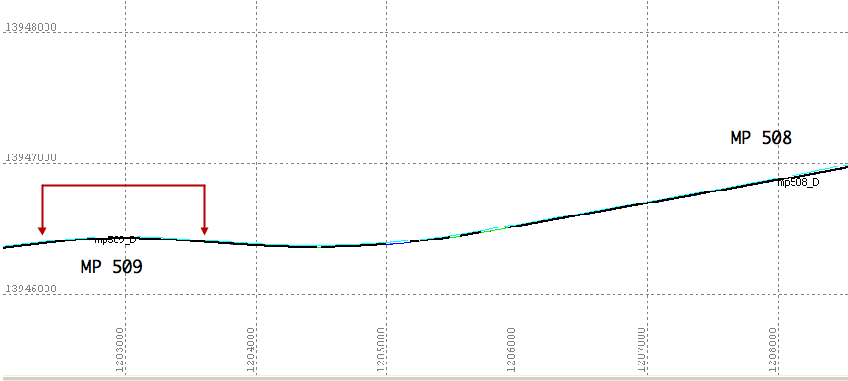
\includegraphics[scale=0.30]{graphics/508_9curve}
	\caption{Plan View MP 508-509}
	\label{crv508_9}
	\end{center}
	\vspace{-10pt}
\end{figure}

\item The track chart indicates the 1 degree curve to the right at mile post 521.15 extends approximately 0.15 miles. The model determined the curve extends from MP 521.15 to 521.83, or one half mile longer than indicated on the track chart. The model determined value is verified by examination of a plan view of the track observations between MP 521 and 522, as illustrated by figure \ref{crv521}.

\begin{figure}[!ht]
	\begin{center}
	\vspace{0pt}
	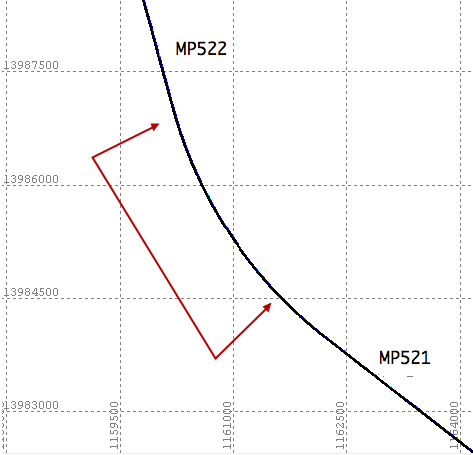
\includegraphics[scale=0.30]{graphics/521-522curve}
	\caption{Plan View MP 521-522}
	\label{crv521}
	\end{center}
	\vspace{-10pt}
\end{figure}

\end{itemize}

Features causing loss of GNSS signal (LOS) were documented by referencing the location on the rail company track chart. When not evident from the track chart, the geodetic coordinates of a point before LOS was entered into Google Maps, and the aerial image examined. This method aided in determining the location of signal bridges and several overpasses not indicated on track charts.

Table \ref{tab:Hi-RailTraverse} also references rail company track chart (TC) values for ${D_c}$ and mile length for comparison with the model output. Track charts do not provide exact values for individual tracks, therefore the comparison serves only to verify the quantity and magnitude of alinement features.

\begin{center}
% Setup for longtable
\begin{longtable}{c l c l}
\caption[RTK Hi-Rail Traverse MP 494-523]{RTK Hi-Rail Traverse MP 494-523}
\label{tab:Hi-RailTraverse} \\
%This is the header for the first page of the table...
\hline
   \multicolumn{1}{c}{\textbf{MP Reference}} &
   \multicolumn{1}{l}{\textbf{Feature}} &
   \multicolumn{1}{c}{\textbf{TC Value}} &
   \multicolumn{1}{l}{\textbf{Note}} \\
\hline
\endfirsthead

%This is the header for the remaining page(s) of the table...
\multicolumn{4}{c}{{\tablename} \thetable{} -- Continued} \\[0.5ex]
\hline
   \multicolumn{1}{c}{\textbf{MP Reference}} &
   \multicolumn{1}{l}{\textbf{Feature}} &
   \multicolumn{1}{c}{\textbf{TC Value}} &
   \multicolumn{1}{l}{\textbf{Note}} \\
\hline
%  \\[-1.8ex]
\endhead

%This is the footer for all pages except the last page of the table...
\midrule
\multicolumn{4}{r}{{Continued next page\ldots}} \\
\endfoot

%This is the footer for the last page of the table...
\bottomrule
\endlastfoot
494-495 & mile length & 8,858' &  Hi-Rail:8,949' \\
	494.05&curve&$3^{\circ}$03'R&\\
	494.46&curve&$2^{\circ}$45'L&\\
	494.65&curve&$2^{\circ}$30'R&\\
495-496 & mile length & 5,295' &  Hi-Rail:5,414' \\
	495.05&curve&$2^{\circ}$30'R&\\
	495.46&curve&$2^{\circ}$30'L&\\
	495.6-495.7&I-64 overpass&&LOS\\
\hline
496-497 & mile length & 5,255' &  Hi-Rail: 5,323' \\	
	496.05&curve&$3^{\circ}$45'L&\\
	496.25&curve&$1^{\circ}$00'L&\\
497-498 & mile length & 5,276' &  Hi-Rail: 5,340' \\
	497.3&curve&$0^{\circ}$45'L&\\
	497.61& & & LOS, VRS update\\
498-499 & mile length & 5,290' &  Hi-Rail: 5,342' \\
	498.6&curve&$2^{\circ}$00'R&\\
499-500 & mile length & 5,283' &  Hi-Rail: 5,342' \\
500-501 & mile length & 5,280' &  Hi-Rail: 5,356' \\
	500.4&curve&$2^{\circ}$32'R&\\
\hline
	501.03-501.12&cross over&&cross over, track 1 to 1\\
	501.15-501.35&Guyandotte River Bridge&&LOS\\
	501.35&curve&$4^{\circ}$14'L&\\
	501.6-501.67&29th Street overpass&&LOS\\
	501.9&curve&$1^{\circ}$33'L&\\
	501.95&curve&$1^{\circ}$33'R&\\
501-502 & mile length & 5,266' &  Hi-Rail: 5,316' \\
	502.62-502.69&cross over&&track 2 to 1\\
502-503 & mile length & 5,383' &  Hi-Rail: 5,208' \\
	503.4&curve&$1^{\circ}$15'L&\\
	503.55&curve&$1^{\circ}$33'R&\\
504-505 & mile length & 5,196' &  Hi-Rail: 5,281' \\
	504.05&curve&$2^{\circ}$56'R&\\
	504.15&curve&$4^{\circ}$30'L&\\
	504.52&curve&$0^{\circ}$55'R&\\
	504.6&curve&$1^{\circ}$05'L&\\
	504.85&curve&$2^{\circ}$00'L&\\
	504.92-504.96&signal bridge&&LOS\\
505-506 & mile length & 5,286' &  Hi-Rail: 5,335' \\
	505.0&spiral&from $2^{\circ}$00'L&\\
	505.5&curve&$1^{\circ}$00'R&LOS@505.55\\
\hline
506-507 & mile length & 5,189' &  Hi-Rail: 5,256' \\
	506.24&curve&$0^{\circ}$32'L&\\
	506.34-506.41&17th Street interchange&&LOS\\
	506.7-507.78&signal bridge&&LOS\\
	506.78&curve&$1^{\circ}$55'R&\\
507-508 & mile length & 5,255' &  Hi-Rail: 5,327' \\
	507.95&curve&$0^{\circ}$23'R&\\
508-509 & mile length & 5,262' &  Hi-Rail: 5,337' \\
	508.37-508.57&Spring Valley Road overpass&&LOS\\
	508.57&curve&$0^{\circ}$45'R&\\
	508.65&signal bridge&& LOS \\
	508.9&curve&$1^{\circ}$18'R&TC error, left\\
509-510 & mile length & 5,280' &  Hi-Rail: 5,355' \\
	509.0&spiral&$1^{\circ}$18'R  & TC in error, left\\
	509.21&curve&$0^{\circ}$18'L&\\
	509.56&curve&$0^{\circ}$28'L&\\
510-511 & mile length & 5,280' &  Hi-Rail: 5,336' \\
	510.2&curve&$1^{\circ}$05'R&\\
	510.7&curve&$3^{\circ}$23'R&\\
	510.95&signal bridge& &LOS\\
\hline
511-512 & mile length & 5,231' &  Hi-Rail: 5,319' \\
	511.72-511.8&Norfolk Southern overpass&&LOS\\
512-513 & mile length & 5,249' &  Hi-Rail: 5,349' \\
	512.52-513&Big Sandy River Bridge&&LOS\\
513-514 & mile length & 5,264' &  Hi-Rail: 5,408' \\
	513.0&curve&$4^{\circ}$51'R&\\
	513.31&signal bridge& &multipath\\
	513.6&curve&$6^{\circ}$23'L&\\
	513.7&curve&$3^{\circ}$00'R&\\
	513.92&curve&$3^{\circ}$00'L&\\
514-515 & mile length & 5,263' &  Hi-Rail: 5,293' \\
	514.0   &curve&$3^{\circ}$00'L& \\
	514.2   &curve&$2^{\circ}$00'R& \\
	514.8   &curve&$2^{\circ}$00'L& \\
	514.55 &signal bridge& &LOS\\
515-516 & mile length & 5,240' &  Hi-Rail: 5,318' \\
	515.0 &curve&$0^{\circ}$45'L& \\
	515.2 &curve&$1^{\circ}$30'R& \\ 
	515.5 &curve&$1^{\circ}$15'R& \\
	515.6 &signal bridge& &LOS\\
	515.8 &curve&$0^{\circ}$45'L& \\
\hline
516-517 & mile length & 5,047' &  Hi-Rail: 5,110' \\	
	516.12&curve&$3^{\circ}$00'R&\\
	516.78-517&curve&$1^{\circ}$00'L&LOS\\
517-518 & mile length & 5,432' &  Hi-Rail: 5,530' \\
	517.0&curve&$1^{\circ}$00'L & to $3^{\circ}$00'L\\
	517.43&curve&$1^{\circ}$30'L&\\
	517.6&curve&$4^{\circ}$15'L&\\
518-519 & mile length & 5,733' &  Hi-Rail: 5,821' \\
	518.05&curve&$1^{\circ}$00'R&\\
	518.23&curve&$1^{\circ}$15'L&\\
	518.4&curve&$0^{\circ}$00'&<sic>\\
	518.41&signal bridge& &multipath\\
	518.5&curve&$0^{\circ}$45'R&\\
519-520 & mile length & 4973' &  Hi-Rail: 5,059' \\
	519.1&curve&$1^{\circ}$30'L&\\
	519.15-519.34&2 signal bridges & &LOS\\
	519.2&curve&$1^{\circ}$00'R&\\
	519.6&curve&$2^{\circ}$00'L&\\
	519.65&curve&$2^{\circ}$00'R&\\
	519.8&curve&$2^{\circ}$30'L&\\
	519.9&curve&$1^{\circ}$45'R&\\
520-521 & mile length & 5,322' &  Hi-Rail: 5,431' \\
	520.5&curve&$2^{\circ}$15'R&\\
	520.55-520.69&Armco overpass& &LOS\\
\hline
521-522 & mile length & 4,972' &  Hi-Rail: 5,357.6' \\
	521.12-521.82&curve&$1^{\circ}$00'R&TC curve length error\\
522-523 & mile length & 5,023' &  Hi-Rail: 5,099' \\
	522.1-522.25&AK Steel Entrance Rd&&LOS\\
	522.6&curve&$1^{\circ}$00'L&\\
	522.9&curve&$0^{\circ}$30'L&\\
\end{longtable}
\end{center}
\vspace{-30pt}

% Measure method comparison between GMRS and Hi-Rail
Measurements obtained from CSX for a GMRS inspection vehicle were compared with the output from the string line model using observations from a RTK GNSS equipped Hi-Rail. The two methods traversed CSX C\&O Ohio Subdivision between mile post 211 and 207. Illustration \ref{fig:gmrs_HiRail} provides a graphic solution to the smoothed $D_c$ vs. mile post values obtained from both methods across the tangent segment.

\begin{center}
\begin{longtable}{c c c c}
\caption[GMRS \& RTK Hi-Rail Comparision, MP 211-207, Alinement Annotation]{GMRS \& RTK Hi-Rail Comparision, MP 211-207, Alinement Annotation}
\label{tab:gmre_Hi-RailTrav} \\
%This is the header for the first page of the table...
\hline
   \multicolumn{1}{c}{\textbf{MP Reference}} &
   \multicolumn{1}{c}{\textbf{Feature}} &
   \multicolumn{1}{c}{\textbf{TC Value}} &
   \multicolumn{1}{c}{\textbf{Note}} \\
\hline
\endfirsthead

%This is the header for the remaining page(s) of the table...
\multicolumn{4}{c}{{\tablename} \thetable{} -- Continued} \\[0.5ex]
   \multicolumn{1}{c}{\textbf{MP Reference}} &
   \multicolumn{1}{c}{\textbf{Feature}} &
   \multicolumn{1}{c}{\textbf{TC Value}} &
   \multicolumn{1}{c}{\textbf{Note}} \\
\hline
%  \\[-1.8ex]
\endhead

%This is the footer for all pages except the last page of the table...
\midrule
\multicolumn{4}{r}{{Continued next page\ldots}} \\
\endfoot

%This is the footer for the last page of the table...
\bottomrule
\endlastfoot
	211-210 & mile length & 5,328' & GMRS:5,018' Hi-Rail:5,368' \\
	210.7     & curve &$2^{\circ}$15'L &\\
	210-209 & mile length & 5,263' & GMRS:4,973' Hi-Rail:5,314' \\
	209.6     & curve &$1^{\circ}$15'L &\\
	209.15   & curve &$1^{\circ}$00'L &\\
	209-208 & mile length & 5,252' & GMRS:5,027' Hi-Rail:5,318' \\
	208.8     & curve &$3^{\circ}$15'R &\\
	208.45   & curve &$1^{\circ}$15'L &\\ 
	208.0     & curve &$3^{\circ}$00'R &\\ 
	208-207 & mile length & 5,678' & GMRS:5,384' Hi-Rail:5,586' \\
	207.5     & curve &$5^{\circ}$00'R &\\ 
\end{longtable}
\end{center}
\vspace{-20pt}

The longest tangent portion of the segment under study extends from MP 210.4 to 209.75, and was selected to determine the variance for the GMRS and the Hi-Rail RTK methods of determining $D_c$ . An ideal measurement over an ideal tangent would result in an instantaneous $D_c$ value of zero at each point of measurement. Assuming the 201.4-209.75 segment as an ideal tangent, the variation around zero $D_c$ was determined for each method. Figures \ref{fig:gmrsVShirail} and \ref{fig:gmrs_HiRail} illustrate the raw and smoothed $D_c$ vs. Mile Post values, while table \ref{tab:tanComp} provides descriptive statistics for $D_c$ values derived from each method. 

\begin{figure}[!h]
	\begin{center}
	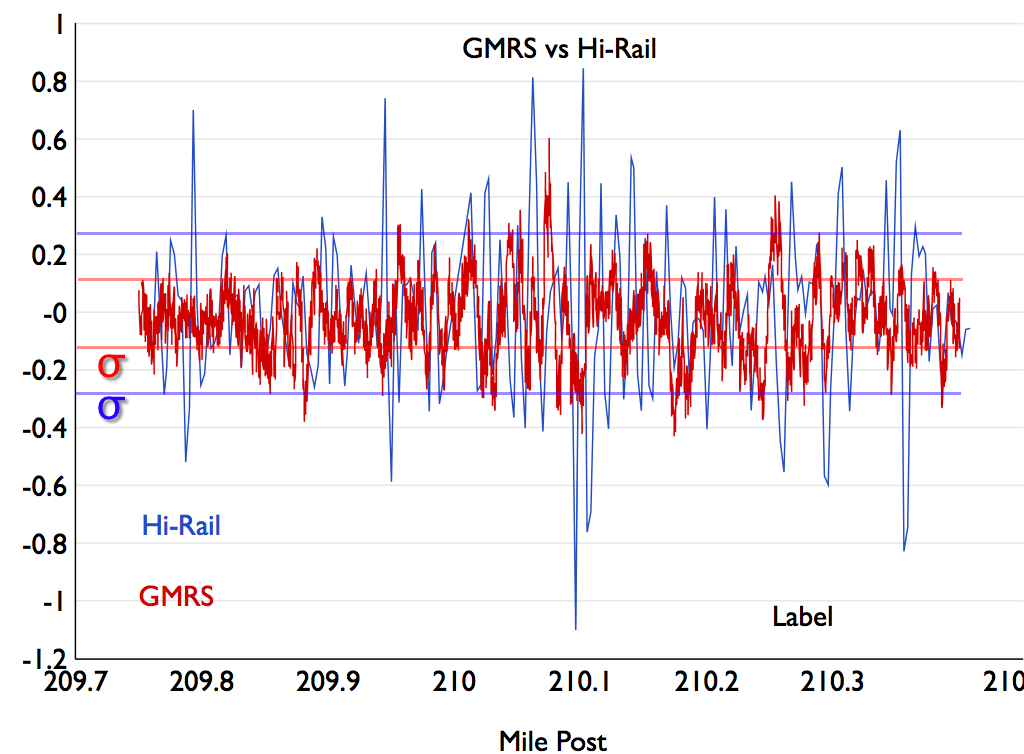
\includegraphics[scale=0.35]{graphics/HiRailVTGC}
	\caption{GMRS and Hi-Rail, $D_c$ Comparison}
	\label{fig:gmrsVShirail}
	\end{center}
\end{figure}

\begin{figure}[!h]
	\begin{center}
	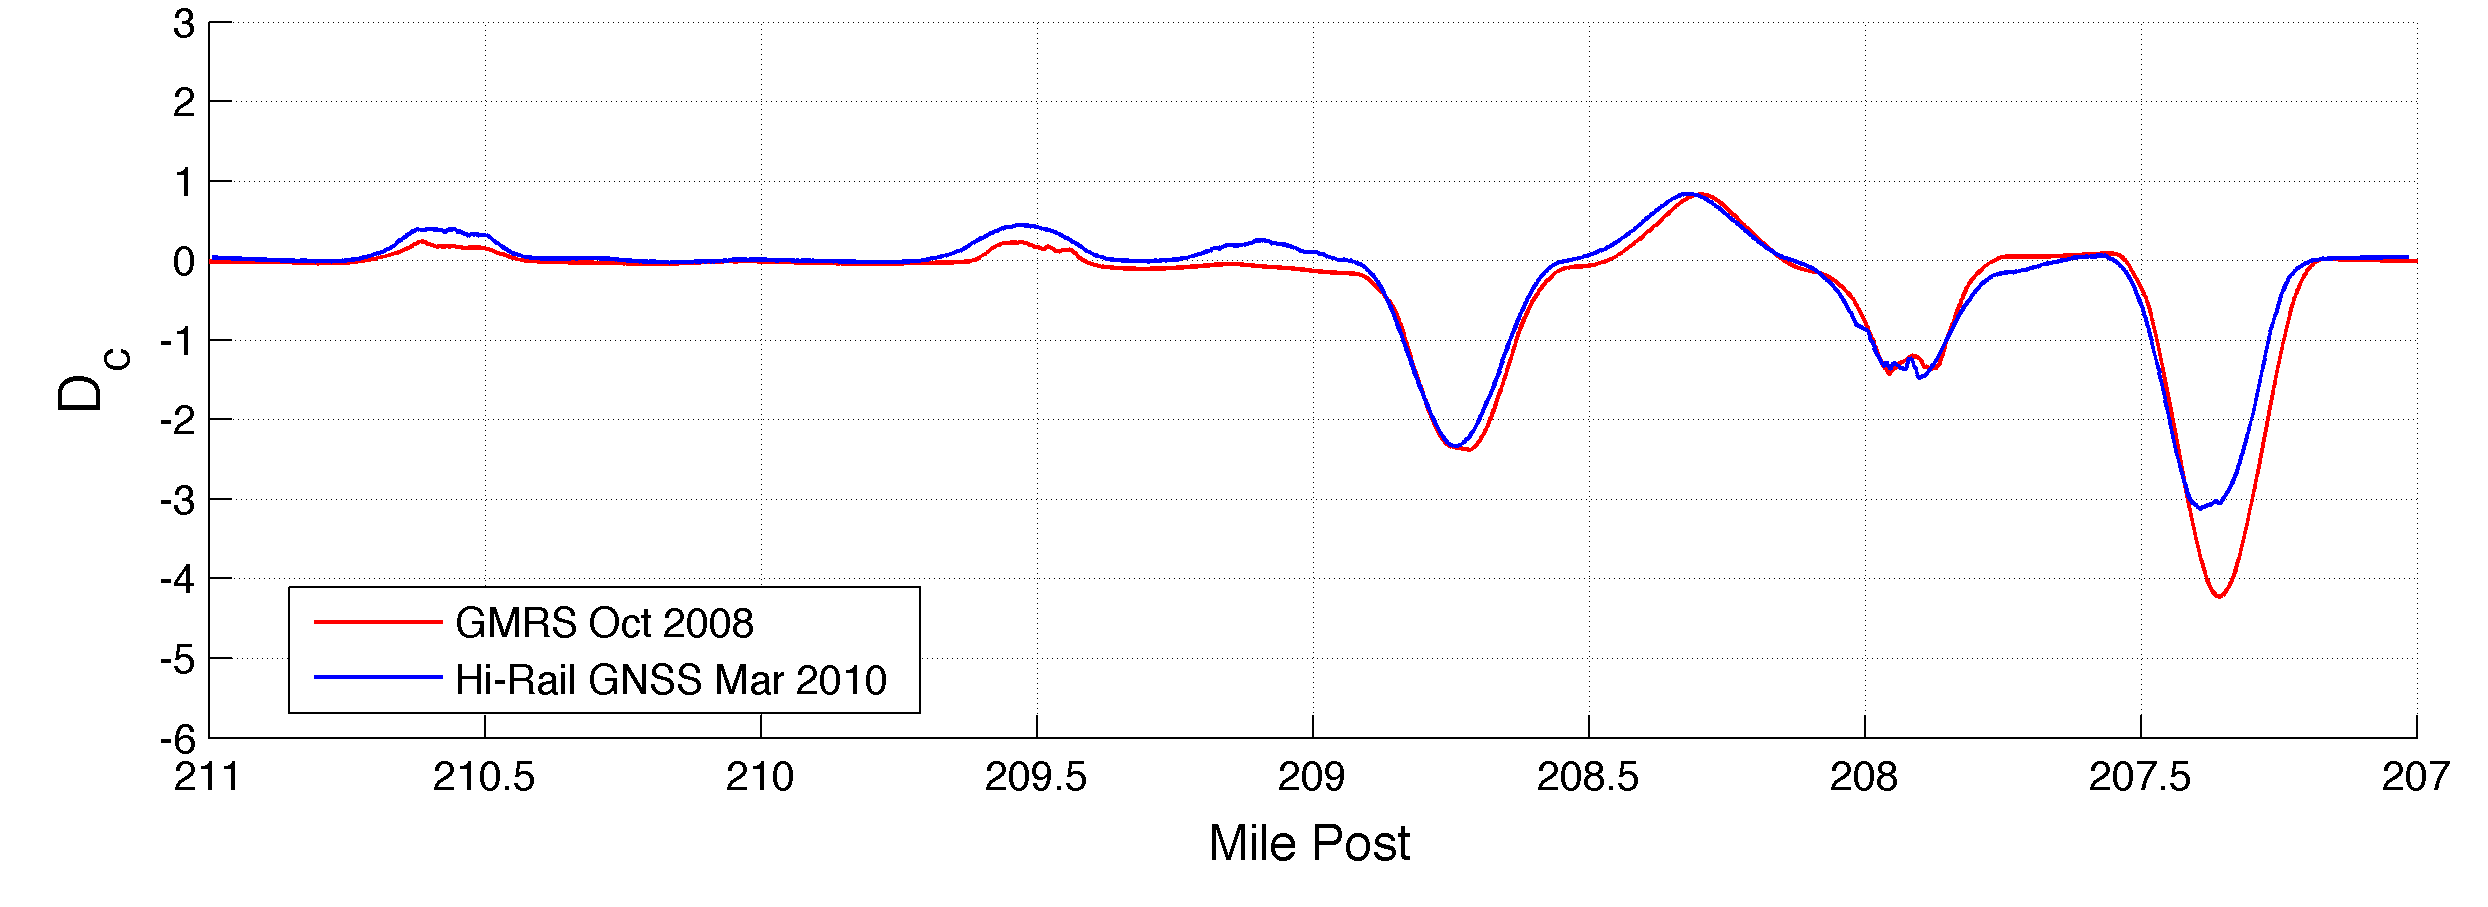
\includegraphics[scale=0.60]{graphics/GMRS_HiRail}
	\caption{GMRS and Hi-Rail, $D_c$ Comparison with Smoothing}
	\label{fig:gmrs_HiRail}
	\end{center}
\end{figure}

\begin{table}
\begin{center}
\caption{GMRS and RTK GNSS Hi-Rail Comparison, MP210.4-209.75 tangent}
\label{tab:tanComp}
\begin{tabular}{c c c c c c c}
\toprule
Vehicle&Stationing&N&${\mu}_{D_c}$&95\% CI&${\sigma}_{D_c}$&95\% CI\\
\midrule
GMRS&1 ft     &3,253&-0.0264&  -0.031  -0.022&0.131&   0.128   0.134\\
Hi-Rail&15.5 ft&222   &-0.0042&-0.0411  0.0327&0.279&0.255   0.308\\
\bottomrule
\end{tabular}
\end{center}
\end{table}

A histogram approximates the probability destiny function of the ${D_c}$ values. GMRS measurement deviation from zero is illustrated in figure \ref{gmrs_hist}. RTK GNSS Hi-Rail deviation illustrated in figure \ref{Hi-Rail_hist}.

\begin{figure}[!h]
	\begin{center}
	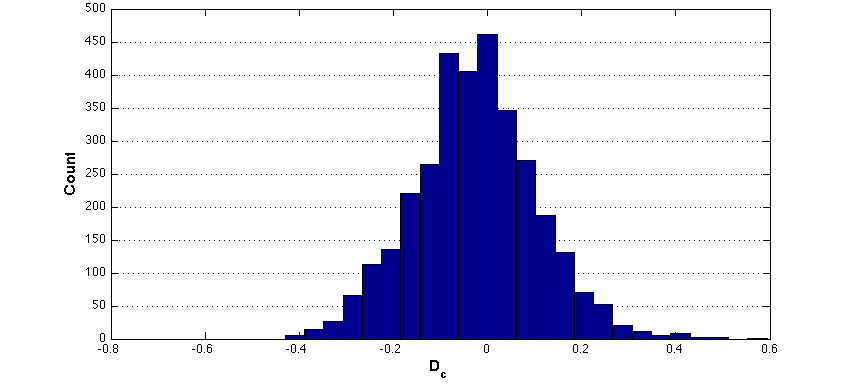
\includegraphics[scale=0.50]{graphics/GMRS_tanHist}
	\caption{GMRS ${D_c}$ Histogram, 210.4 to 209.75 tangent}
	\label{gmrs_hist}
	\end{center}
\end{figure}

\begin{figure}[!h]
	\begin{center}
	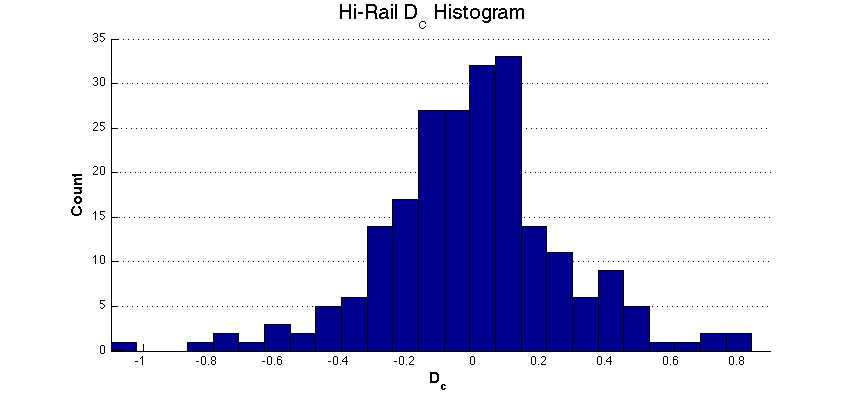
\includegraphics[scale=0.50]{graphics/HiRail_tanHist}
	\caption{Hi-Rail ${D_c}$ Histogram, 210.4 to 209.75 tangent}
	\label{Hi-Rail_hist}
	\end{center}
\end{figure}

%\clearpage 

%Track Occupancy Results
\section{Track Occupancy Results}
The question answered by experiment 3 was whether statistical evidence exists to determine if a wireless positioning system can act as the sole track vehicle location determination system capable of meeting FRA guidelines for track occupancy as might be used as a location determination system in positive train control.

The question was answered through the completion of several objectives:
\begin{itemize}
\item An analytical method was developed to determine the variance in a series of RTK GNSS measured track positions from specific geometric segments surveyed by a common track vehicle.
\item A hypothesis test determined the likelihood of RTK GNSS position measurements in tangents and circular curves to meet the FRA criteria for reliable track occupancy.
\end{itemize}

Table \ref{tab:tanRegress} presents the result of a linear least squares regression performed on Easting and Northing coordinate pairs between mile post reference 498.9 and 500.2 for each of five traverses. Track position observations traversing three parallel tangent tracks of the same approximate length were recorded during five separate surveys, denoted as traverses A-E. The regression correlation statistic ${R^2}$ for each traverse was 0.99998 or better.

\begin{table}[!h]
	\begin{center}
	\caption{Tangent Regression Coefficients, MP 498.9 to 500.2}
	\label{tab:tanRegress}
		\begin{tabular}{c c c c c c c}
\toprule
%\multicolumn{3}{l}{$\alpha = 0.00001$}\\
	Survey & Track & N  & Slope  & Y Intercept & Variance & Azimuth$^{\circ}$\\
\midrule
	A & 2 & 1,189 & 0.10220 & 13825809.25 & 0.02259 & 264.1645$^{\circ}$\\
	B & 2 & 1,244 & 0.10219 & 13825815.49 & 0.02208 & 264.1648$^{\circ}$\\
	C & 3 & 1,152 & 0.10208 & 13825969.10 & 0.05664 & 264.1711$^{\circ}$\\
	D & 1 & 1,158 & 0.10214 & 13825873.25 & 0.02432 & 264.1680$^{\circ}$\\
	E & 3 & 1,156 & 0.10210 & 13825950.11 & 0.05338 & 264.1703$^{\circ}$\\
	\bottomrule
	\end{tabular}
	\end{center}
\end{table}

The cross-track error was determined for each point surveyed and a centerline described from the regression coefficients of traverse A. Descriptive statistics for the cross-track distance from each point to the reference centerline for each survey is presented in table \ref{tab:tanRegress}.
% Hypothesis test
\needspace{3\baselineskip}

Table \ref{tab:tanHypo} provides the result of the tangent case hypothesis test for each traverse between MP 498.9 and 500.2, with \emph{N} the number of data points, $\mu_{xt}$ the mean cross track distance of the traverse in feet, and ${\sigma_{xt}}$ the standard deviation.

\begin{table}[!h]
	\begin{center}
	\caption{Tangent Cross-Track Hypothesis Test}
	\label{tab:tanHypo}
		\begin{tabular}{c c c c c }
\toprule
{$\alpha = 0.00001$} & & & &\\
	$Track_{trav}\rightarrow Track_{ref}$ & N   & ${\mu_{xt}}$ & ${\sigma_{xt}}$ & Reject ${h_0}$?  \\
\midrule
	 $2_A\rightarrow2_A$ & 1,189   & 0.13  & 0.075   & no \\
	 $2_B\rightarrow2_A$ & 1,244   & 0.13  &  0.080  & no \\
	 $3_B\rightarrow2_A$ & 1,152   & 13.10    &  0.347  & yes \\
	 $1_B\rightarrow2_A$ & 1,158   & 13.51    &  0.203  & yes \\
	 $3_B\rightarrow2_A$ & 1,156   & 13.05    & 0.313   & yes \\
\bottomrule
	\end{tabular}
	\end{center}
\end{table}
	
\begin{table}[!h]
	\begin{center}
	\caption{Curve Regression Coefficients, MP 500.5 to 500.7}
	\label{tab:crvRegress}
		\begin{tabular}{c c c c c c c}
\toprule
\multicolumn{3}{l}{A radius = 2276.11ft} \\
	Survey & Track & N  & Origin E  & Origin N & ${\mu_{xt}}$ & ${\sigma_{xt}}$\\
\midrule
	A & 2 & 85 & 1245217.14 & 13955358.41 & 0.00 & 0.033 \\
	B & 2 & 98 & 1245215.55 & 13955352.03 & 0.03  & 0.037 \\
	C & 3 & 98 & 1245203.52 & 13955318.38 & -14.53   & 0.163 \\
	D & 1 & 97 & 1245207.64 & 13955326.35 & 13.93    & 0.095 \\
	E & 3 & 92 & 1245206.38 & 13955328.18 & -14.57   & 0.142 \\
	\bottomrule
	\end{tabular}
	\end{center}
\end{table}

Table \ref{tab:crvHypo} provides the result of the circular curve hypothesis test for each survey between MP500.5 and 500.7.

\begin{equation}
	h_{0}: \mu_{xt} < \frac{11.5}{2}
\end{equation}
\begin{equation}
	h_{1}: \mu_{xt} \ge \frac{11.5}{2}
\end{equation}

\begin{table}[!h]
	\begin{center}
	\caption{Circular Curve Cross-Track Hypothesis Test}
	\label{tab:crvHypo}
		\begin{tabular}{c c  c c c }
\toprule
{$\alpha = 0.00001$} & &   &\\
	$Track_{trav}\rightarrow Track_{ref}$ & N  & ${\mu_{xt}}$ & ${\sigma_{xt}}$ & Reject ${h_0}$?  \\
\midrule
	 $2_A\rightarrow2_A$ & 85   &  0.00 & 0.033  & no \\
	 $2_B\rightarrow2_A$ & 98   &   0.03  & 0.037  & no \\
	 $3_C\rightarrow2_A$ & 98   &  -14.53    & 0.163  & yes \\
	 $1_D\rightarrow2_A$ & 97   &   13.93      & 0.095  & yes \\
	 $3_E\rightarrow2_A$ & 92   &   -14.57     & 0.142  & yes \\
\bottomrule
	\end{tabular}
	\end{center}
\end{table}

% Summary
\section{Summary}
Experiment 1 traversed an active hump yard with a locomotive equipped with RTK GPS instruments to observe track positions. The recorded positions were used to produce a profile for each track. Reference benchmarks, evaluation of GPS signals at the reference station, a plan view of the yard with color-mapped elevations, a plan view of the relative vertical error, and 58 track profiles are exhibited in Appendix A. The relative vertical precisions of locomotive and reference station observations were examined for the influence of multipath reflections. 

Experiment 2 traversed a continuous 29 mile segment of mainline track by a Hi-Rail equipped with RTK GNSS instruments. A model of the string line method was used to determine the ${D_c}$ for each mile, evaluate the model against rail company track charts for location, magnitude, and direction of curves. The model was used to evaluate the model output against a specialized track geometry car over a comparable segment of tangent track. Company track charts, the output of the string line model for each mile, and the model script is exhibited in Appendix B.

Experiment 3 evaluated the ability to determine track occupancy by RTK GNSS. Five surveys traversed a parallel multitrack segment. The cross-track error between a baseline survey and subsequent surveys was evaluated in a tangent and circular curved segment. The statistical likelihood of estimating track occupancy meeting FRA guidelines for a location determination system was determined.
	% !TEX root = dissertation2.tex
\chapter{Conclusions}
This chapter contains a summary of the purpose, procedures, major findings, conclusions and discussion, recommendations, and implications of the research.

% Purpose
\section{Purpose}

The researcher explored track measurement using commercial off-the-shelf instrumentation to observe railway positions. The research examines a system for track surveying that minimizes exposure to railway hazards, is cost-effective, and produces accurate repeatable measurements without burdening train movement authority or disrupting yard operations, answering these questions:

1)\emph{Hump Yard Profile:}
Can a locomotive use wireless position measurement to determine the vertical profile of bowl tracks in an automatic classification yard to an accuracy of tenth of a foot during production activities?

2)\emph{Horizontal Track Alinement:}
Can a common track vehicle use wireless position measurement to determine the horizontal degree of curvature ($D_c$) comparable with specialized track geometry vehicles?

3)\emph{Track Occupancy:}
Can a common track vehicle use wireless position measurement to meet the positioning requirements for track occupancy outlined by the FRA~\citep[pp.6-7]{1995FRADiffe} for a location determination system?

% Procedures
\section{Procedures}

The researcher conducted three experiments which used common track vehicles equipped with COTS GNSS survey instruments. To observe track position, a single RTK antenna and receiver were mounted to a locomotive in the case of the hump yard, or to a Hi-Rail in the case of mainline track. Correctors were transmitted to a mobile receiver using two methods; a VHF data radio in the case of the humpyard; and the public cellular network in the case of mainline track. No auxiliary instrumentation was used to modify observations or fill expected data gaps.

% Experiment one procedures
\begin{enumerate} 
\item Experiment 1 traversed an active hump yard with a locomotive equipped with an RTK GPS instrument. Observed track positions were used to produce a profile for each track. The relative vertical precision of the locomotive observations and the reference station observations were examined for the influence of multi-path signal reflections. Experiment 1:

\begin{itemize}
	\item Developed a procedure for aligning a GPS antenna mounted to a locomotive with the track  centerline top-of-rail location.
	\item  Collected continuous single epoch observations on a nominal 10 foot horizontal spacing with RTK augmented GPS onboard a locomotive in an active hump yard. 
	\item Produced a plan-view color-map of track elevation for the bowl area of a hump yard.
	\item Produced a two-dimensional profile drawings for each track in 1:1 and 1:5 vertical scale.
	\item Produced a plan-view color-map of relative vertical precision as determined by the \emph{Survey Controller} software for points measured in the bowl area of the yard.
	\item Determined the descriptive statistics of the relative vertical precision estimate as determined by \emph{Survey Controller} software for the locomotive mounted GPS.
	\item Produced a TEQC report for the ad hoc reference station during an observation session for the purpose of determining clock resets due to multi-path GPS signal reflection.
\end{itemize}

% Experiment two procedures
\item Experiment 2 traversed a 29 mile segment of mainline track by an inspector's Hi-Rail equipped with RTK GNSS instruments. A software model was used to determine the degree of curvature (${D_c}$). The model output was verified against rail company track charts for location, magnitude, and direction of track features. The model was used to evaluate the performance of RTK GNSS against a specialized track geometry car across tangent track. Experiment 2:
\begin{itemize}
	\item Developed a procedure for aligning a GNSS antenna mounted to a Hi-Rail with the track centerline top-of-rail location.
	\item Developed a procedure for RTK measurement by Hi-Rail across mainline track.
	\item Developed a software model of the string line method as described by the FRA \emph{Track Safety Standards Compliance Manual}.~\citep{2007FRATrack}
	\item Compared the model output from RTK Hi-Rail inputs with company track charts. The comparison between the model and track charts was verified for curve location, magnitude, and location. Mile length determined by the model was compared with the published track chart mile length.
	\item Produced descriptive statistics for $D_c$ variation across a tangent segment for a track geometry car and RTK Hi-Rail modeled $D_c$.
	\item Produced a graphic solution for comparing $D_c$ measured by geometry car and RTK equipped Hi-Rail by plotting $D_c$ vs. mile post reference.
	\item Determined the variability of $D_c$ as measured by a geometry car and RTK equipped Hi-Rail across tangent track.
\end{itemize}

% Experiment three procedures
\item Experiment 3 evaluated the ability of RTK GNSS to determine track occupancy. Five surveys traversed a parallel multitrack section of mainline track. The cross-track error between a baseline survey and subsequent surveys was evaluated in both a tangent and circular curved segments. The statistical likelihood of estimating track occupancy meeting FRA guidelines for a location determination system was determined. Experiment 3:

\begin{itemize}
\item Observed track positions for three parallel tracks by RTK GNSS equipped Hi-Rail.
\item Determined the coefficients for a reference tangent and circular track centerlines from an initial traverse.

\item Determined the cross-track error between subsequent RTK Hi-Rail observations and the reference tangent curve centerline.

\item Determined by hypothesis test if statistical evidence exists to indicate if RTK GNSS is capable of determining track occupancy meeting FRA performance standards for a location determination system.
\end{itemize}
\end{enumerate}
% Major findings
\section{Major Findings}

The research answered the questions:
 
\begin{enumerate}

% Major findings, hump yard survey
\item Can a locomotive use wireless position measurement to determine the vertical profile of bowl tracks in an automatic classification yard to an accuracy of tenth of a foot during production activities?

The experiment was successful in using a single reference station located at the rail terminal with a RTK equipped locomotive to define the grades of 58 tracks in an automatic classification yard during production activity to a mean relative vertical accuracy of 0.078 feet.
\begin{itemize}
\item The hump yard profile survey resulted in a ground hazard exposure of six man-hours.
\item The hump yard profile survey resulted in ten thousand single epoch observations.
\item The hump yard profile survey was completed in 5 working days.
\item The hump yard profile survey cost 100 man hours and 4-1/2 locomotive shifts.
\item The hump yard profile survey interrupted humping operations for less than 2 hours.
\item Distortions from multi-path reflection were not detected. 
\end{itemize}

% Major findings, track alinement
\item Can a common track vehicle in using networked RTK GNSS to determine the horizontal degree of curvature ($D_c$) comparable with specialized track geometry vehicles?

The experiment was successful in determining $D_c$ from measurements utilizing a track inspector's Hi-Rail equipped with a RTK GNSS instrument. Correctors received from a state sponsored VRS network transmitted through a public cellular network provided continuous coverage across 29 miles of mainline track.

The comparison of $D_c$ between the X,Y,Z coordinates modeled from a RTK GNSS traverse by Hi-Rail and a specialized track geometry car over an identical segment of tangent track were comparable in terms of approximate result. However, the $D_c$ standard deviation modeled from RTK X, Y, Z coordinates was twice the valus as the $D_c$ standard deviation obtained from the CSX GMRS-1 track geometry car.

\begin{itemize}
\item Five traverses of multiple parallel track resulted in 97,180 single epoch observations.
\item The software model determined ${D_c}$ by 62 foot chords and 15.5 foot stations. The model output compared favorably with published rail company track charts.
\item Data gaps in the model output were identified. Each obstruction was identified as a fixed overhead structure such as a highway overpass, bridge superstructure, or signal bridge.
\item RTK ${D_c}$ measurements by Hi-Rail across a tangent track segment were found to have a 2${\sigma}$ confidence interval of the mean between -0.041 and 0.033 feet, with a standard deviation of 0.279 feet. The CSX GMRS-1 track geometry car traversing the identical tangent segment was found to have a 2${\sigma}$ confidence interval of the mean between -0.031 and -0.022 feet with a standard deviation of 0.131 feet.
\end{itemize}

% Major findings, track occupancy
\item Can a common track vehicle use wireless position measurement to meet the positioning requirements for track occupancy outlined by the FRA~\citep[pp.6-7]{1995FRADiffe} for a location determination system?

The experiment was successful in using RTK GNSS to meet the wireless positioning guidelines for a location determination system (LDS). Track occupancy between three parallel tracks, in tangent and circular curve segments, was determined within the significance level suggested by the FRA.

\begin{itemize}
\item Track occupancy was determined between three parallel tracks by five traverses of a RTK GNSS equipped Hi-Rail.
%tangent
\item The coefficients describing the reference tangent on track 2 between MP498.9 and 500.2 were determined to have a slope of  0.1022017 (azimuth = 264.1645$^{\circ}$) and a Y-intercept of 13825809.25. The ${R^2}$ statistic for the regression was determined to be 0.99998.
\item The mean cross-track error for a traverse of track 2 referencing the track 2 tangent between between MP498.9 and 500.2 was found to be 0.13 feet with a standard deviation of 0.080 feet. The alternate hypothesis $h_{1}: \mu_{xt} \ge \frac{11.5}{2}$ was rejected at a 99.999\% confidence level.
\item The mean cross-track error for a traverse of track 3 referencing the track 2 tangent between between MP498.9 and 500.2 was found to be 13.10 feet with a standard deviation of 0.347 feet. The null hypothesis $h_{0}: \mu_{xt} < \frac{11.5}{2}$ was rejected at a 99.999\% confidence level.
\item The mean cross-track error for a second traverse of of track 3 referencing the track 2 tangent between between MP498.9 and 500.2 was found to be 13.05 feet with a standard deviation of 0.313 feet. The null hypothesis $h_{0}: \mu_{xt} < \frac{11.5}{2}$ was rejected at a 99.999\% confidence level.
\item The mean cross-track error for a traverse of a track of track 1 referencing the track 2 tangent between between MP498.9 and 500.2 was found to be 13.51 feet with a standard deviation of 0.203 feet. The null hypothesis $h_{0}: \mu_{xt} < \frac{11.5}{2}$ was rejected at a 99.999\% confidence level.
%circular curve
\item The coefficients describing the reference circular curve on track 2 between MP500.5 to 500.7 were determined to have an origin located at Northing 13955358.41, Easting 1245217.14 and a radius of 2276.11 feet.
\item The mean cross-track error for a traverse of track 2 referencing the track 2 circular curve between between MP500.5 to 500.7 was found to be 0.03 feet with a standard deviation of 0.037 feet. The alternate hypothesis $h_{1}: \mu_{xt} \ge \frac{11.5}{2}$ was rejected at a 99.999\% confidence level.
\item The mean cross-track error for a traverse of track 3 referencing the track 2 circular curve between between MP500.5 to 500.7 was found to be -14.53 feet with a standard deviation of 0.163 feet. The null hypothesis $h_{0}: \mu_{xt} < \frac{11.5}{2}$ was rejected at a 99.999\% confidence level.
\item The mean cross-track error for a second traverse of track 3 referencing the track 2 circular curve between between MP500.5 to 500.7 was found to be -14.57 feet with a standard deviation of 0.142 feet. The null hypothesis $h_{0}: \mu_{xt} < \frac{11.5}{2}$ was rejected at a 99.999\% confidence level.
\item The mean cross-track error for a traverse of track 1 referencing the track 2 circular curve between between MP500.5 to 500.7 was found to be 13.93 feet with a standard deviation of 0.095 feet. The null hypothesis The null hypothesis $h_{0}: \mu_{xt} < \frac{11.5}{2}$ was rejected at a 99.999\% confidence level.

\end{itemize}
\end{enumerate}

% Conclusions and Discussion
\section{Conclusions and Discussion}
A number of conclusions may be drawn for an analysis of the data generated by the study.
\begin{enumerate}
% Conclusions, hump yard survey
\item 
It may be concluded that the method of using a RTK equipped locomotive to survey an active hump yard was able to measure track elevation with a relative vertical accuracy less than 0.1 feet.

\item 
It may be concluded that the method of using a RTK equipped locomotive to survey an active hump yard is safer than a traditional differential level survey.

The use of a locomotive to survey the yard considerably reduced on-track worker exposure to hazards when compared with a differential level survey. The method of using an RTK locomotive resulted in a ground exposure of 6 man-hours compared with an estimated 500 man-hours for a differential level survey.

\item 
It may be concluded that the method of using a RTK equipped locomotive to survey an active hump yard provides greater observation density than a typical differential level survey.

The nominal observation distance between observations by RTK locomotive was 10 feet compared with the common practice of using 100 foot stations during a traditional differential level survey.

\item 
It may be concluded that the method of using a RTK equipped locomotive to survey an active hump yard reduces time-to-completion from an estimated 4-6 weeks to one week.

A related finding was that the use of a RTK equipped locomotive to survey an active hump yard was unaffected by a full day of torrential rain.

\item 
It may be concluded that the method of using a RTK equipped locomotive to survey an active hump yard reduces labor cost from 500 man-hours to 100 man hours.

\item 
It may be concluded that the method of using a RTK equipped locomotive to survey an active hump yard increases equipment costs by using a locomotive for 36 hours.

A related finding was that the use of a RTK equipped locomotive to survey an active hump yard could use the survey locomotive to pull cuts of cars, kick stalls, and attend to many of the normal duties assigned to a yard engine without affecting track observations.

\item
It may be concluded that the method of using a RTK equipped locomotive to survey an active hump yard interrupted hump operations for less than two hours.

\item
It may be concluded that the reference station and roving receiver used during the locomotive survey of an active hump yard did not exhibit gross positioning errors attributable to multipath signal reflections.

% Conclusions, track alinement
\item
It may be concluded that the use of a RTK equipped Hi-Rail during an inspector's routine visual track inspection had no impact on train operations.

\item 
It may be concluded that the use of a RTK equipped Hi-Rail during an inspector's routine visual track inspection to model ${D_c}$ by the string line method was successfully verified by reference to the location, direction, and ${D_c}$ in company track charts. 

\item
It may be concluded that the use of a RTK equipped Hi-Rail observations modeling ${D_c}$ was not precisely equivalent to the ${D_c}$ determined by the CSX GMRS-1track geometry car.

A related finding was that the track geometry car 95\% confidence interval of the mean over the tangent segment failed to capture zero ${D_c}$. It may be concluded that; either the track geometry car measurement of ${D_c}$ exhibits a slight bias to the left, or that the tangent track segment under study has a slight left curve.

% Conclusions, track occupancy

\item
It may be concluded that, given; a priori track centerline locations determined by RTK GNSS; the use of a network RTK VRS server; RTK GNSS equipped track vehicles; and a method of communicating correctors to a track vehicle, that track occupancy can be determined by single epoch RTK GNSS observation to the accuracy suggested for a wireless determination system by the FRA for a location determination system~\citep[pp.6-7]{1995FRADiffe} .

\end{enumerate}

% Recommendations
\section{Recommendations}
Recommendations for further study, implementation, and improvements regarding the use of RTK GNSS in railroad transportation as a result of research outcomes.

% Hump yard questions
\begin{itemize}
\item
Can track surfacing equipment be adapted to use automated machine guidance methods? It is not unusual in the railroad industry to rely on operator skill and judgment to establish grade during yard wide resurfacing projects. Operator skill and judgement are not data driven, and do not fully take advantage of available technologies, such as RTK GNSS. A track surfacing system, borrowing from the technology present in 3D machine control methods, would produce data-driven guidance for machine operators.

\item
Do improvement in track grade lead to increased yard throughput? In general, grades closer to design reduce the need to resurface as frequency; reduce retarder maintenance; and produce closer to the design coupling speed, in turn reducing damage to draft gear and yard derailments leading to a decrease in yard delay. An analysis of pre-surfacing and post-surfacing hump yard throughput would produce evidence of the contribution of grade deterioration on freight service delay.

\item
How do grade issues affect car handling in flat yards, particularly in light of increasing reliance on remote control locomotive? Flat yards typically handle lower quantities of rail cars than hump yards but share a similar reliance on track grade quality for predictable rail car movement.

% Track alinement questions

\item
Is a string line model the correct method for determining ${D_c}$? String lining is accepted as a standard for measurement of ${D_c}$, and until recently, the only practical method for a track inspector to flag or find alinement exceptions. More computationally efficient methods are available (by deflection angles) for determining ${D_c}$, and might be more readily adapted for real-time determination of ${D_c}$ from RTK GNSS observations.

\item
Is ${D_c}$ the correct measurement for determining track alinement? ${D_c}$ is determined in two dimensions, while the railway guides rolling stock in three dimensions. Modeling the trackway in four dimensions (x, y, z, time) may provide a more comprehensive perspective as shown in \href{http://www.youtube.com/watch?v=mOeuHxUPRBc}{this video}\footnote{http://www.youtube.com/watch?v=mOeuHxUPRBc}. The video fly through of the Hamlet Terminal before resurfacing enables the discovery of relationships between tracks not readily apparent in two dimensional profiles.

\item
Can RTK track observations be considering as a diagnostics tool to provide actionable information for identifying track defects? Additional study and a more refined model for determining ${D_c}$ is required to determine if reliable actionable information can be derived from RTK GNSS track observations for the identification of track alinement defects. The experimental results here indicate that RTK GNSS has the capability to locate defects in track classes 1-4.

\item
How can RTK add value as a change management tool? RTK GNSS provides the ability to ground-truth asset locations determined from LiDAR surveys, and accurately record the work typically performed during track inspections, such as replacing sheared frog bolts or insulated track joints. Further study in recording track maintenance activity over time may provide the ability to perform geographic trend analysis leading to the identification of geologic, alinement, or weather induced factors affecting particular railway segments.

\item
Can RTK be used to observe the behavior of CWR\footnote{Continuously Welded Rail} movement due to seasonal temperature effects? Rail expands and contracts with temperature. Anecdotal evidence of track shift in response to long-term seasonal temperature differences can be quantified through further study of this phenomenon by RTK GNSS.

\item
Can areas of rail breakage or warping\footnote{Aka ``sun kinks''.} be modeled using RTK track observations? Short-term temperature fluctuations that exceed the railway neutral temperature limits impart tensive/compressive forces in the rail. Further study of short-term temperature fluctuation by RTK GNSS may provide sufficient position accuracy to identify factors contributing to this phenomena.

\item
To what extent will GPS Block IIF satellites reduce data dropouts from overhead structures as experienced during experiment 2 mainline surveys? The addition of the L5 signal and higher power (+3db) of the 12 scheduled\footnote{first L5 capable SV launch May 2010} Block IIF and Block III\footnote{First scheduled launch 2013.} satellites will have a positive benefit for RTK users. Further study would indicate the expected improvement in eliminating data dropouts from overhead structures.

\item
Is an RTK GNSS survey by Hi-Rail possible in deep mountain valleys, as in the southern coal fields of West Virginia? Coal accounts for the majority of freight carried by rail ~\citep{RITAtransStats08}. The narrow, steep valleys of southern West Virginia present a challenge for maintaining continuous GNSS and data coverage. Further study could identify the major factors impacting the use of RTK GNSS in similar challenged areas.

% Track Occupancy

\item
Can mobile RTK GNSS, in conjunction with LiDAR derived track centerlines, be used as a basis for a wireless LDS? Class I railroads are flying LiDAR missions over track to quickly produce baseline locations of track and wayside assets in anticipation of meeting PTC regulation by 2015. Further study in looking a the combination of LiDAR derived centerlines with mobile RTK GNSS would establish if the combination is suitable for use as a wireless LDS.

\item
Can RTK enabled locomotives take advantage of the unused bandwidth of wayside repeaters to transmit train location as part of an LDS? Wayside repeaters relay digitized voice packet to rail company movement authority. Unused capacity exists for transmitting other data through existing infrastructure. Additionally, narrow banding requirements by the FCC will double and eventually quadruple the communication channels available in the AAR VHF and UHF bands. Additionally, Class 1 railroads have obtained spectrum in the 220Mhz band for use in PTC.

Further study exploiting existing wayside radio assets for communicating RTK correctors to mobile units would provide knowledge as to the extent and communication demands for covering areas underserved by public wireless or cellular networks.

\item
Is the civilian-use safety-of-life signal from GPS BlockIIF sufficient to insure the use of GPS as part of a vital LDS? New GPS signals beginning with the May 2010 launch of the Block IIF series provide a method to signal users of service interruptions. Research defining the needs and performance these signals would determine the suitability of GNSS as a vital system for PTC.

\item
Can determining the track occupancy of a railcar in transit across a yard assist ``right track, right train'' consist makeup? Correctors transmitted by a rail yard communications system would enable low-cost GPS receivers with sub-meter accuracy.
	
\end{itemize}

% Implications
\section{Implications}

\begin{enumerate}

\item
Hump yard stakeholders can consider the relative safety costs when selecting a survey method in preparation for yard-wide resurfacing or to identify grade problems.

\item
The safety aspects of a yard survey by RTK have implications for yard managers, hump yard engineers, and on-track workers. Personnel safety is improved by removing them from potentially hazardous situations. Track closures and railcar reroutes are not mandatory to determine yard grades.

\item
Increased observation density during a hump yard survey has implications in improving material take-offs estimates and the finished grade quality for yard resurfacing projects.

\item
Increased observation density, combined with a diligent attention to as-build grades during resurfacing, has implications for reducing variability during the humping process.

\item
Reducing time-to-completion for a yard survey is of importance to planners and hump yard engineers in estimating yard survey costs.

\item
The use of a yard trim locomotive is of importance to yard managers in estimating the demand on yard resources in supporting a profile survey.

\item
The low impact on yard operations is of importance to traffic planners, managers, and hump yard engineering management in eliminated unidentifiable costs caused by track closures and car rerouting.

\item
The inability to detect anomalous track position due to multi-path signal reflections is of importance to hump yard engineers by eliminating a potential measurement error source when performing a RTK survey.

\item
Track engineering and maintenance implications in determining track alinement by RTK GNSS provides: the means to deploy commercial off-the-shelf products; an immediately accessible and proven method for monitoring track behavior monitoring. 

\item
Increased track position monitoring frequency has implications for track engineering managers and superintendents in studying the behavior of track and as a method for establishing track asset change management procedures.

\item
Wayside track references rely on established fixed locations for mile post reference positions. Establishing ``virtual mileposts'' has implications for track engineering managers and superintendents in considering how to bridge legacy track reference marks with modern absolute positioning measurement.

\item
With few exceptions, dense CORS networks are available from each  state in the contiguous US, either as a free service or from private for-profit firms. The growing availability of wireless data and the use of localized VHF/UHF or utilization of the unused bandwidth of wayside repeaters removes the usefulness of NDGPS in all but the most remote locations. The wide availability of RTK services has implications for the need for continued funding of NDGPS.

\item
Track location transmitted by rolling stock combined with accurate yard centerlines has implications for hump control systems using continuous rail car occupancy rather than timers and switches or video analytics in determining ``right track, right train'' consist makeup. 

\end{enumerate}

\backmatter
% Include appendices.
	\include{AppendixA}
	\include{AppendixB}
% Bibliography at the end
	\bibliographystyle{plain}% authordate ,apalike,plain(sorted),unsrt(unsorted),alpha plain,abbrv,acm,unsrtnat, plainnatbib
		% natbib styles: unsrtnat.bst, plainnat.bst, abbrvnat.bst
	\bibliography{Dissertation}
\end{document}